\documentclass[12pt]{article}
\usepackage[a4paper, margin=.9in]{geometry}
% \usepackage{xeCJK}
% \setCJKmainfont{Microsoft YaHei} 
\newcommand{\DOUBLECOL}{}	% turns this on for double column
\newlength{\subfigureheight}
\newlength{\figurewidth}
\ifdefined\DOUBLECOL
\setlength{\subfigureheight}{2.45in}
\setlength{\figurewidth}{3.5in}
\else
\setlength{\subfigureheight}{2.35in}
\setlength{\figurewidth}{6.5in}
\fi
\usepackage{amsfonts,amsmath,amssymb,bm,cancel,color,comment,epsfig,enumerate,empheq,floatrow,hyperref,mathdots,mathrsfs}
\usepackage{placeins}%\usepackage{algorithmic}
\usepackage[vlined,ruled,linesnumbered]{algorithm2e}
\SetKwInput{KwInput}{Input}                % Set the Input
\SetKwInput{KwOutput}{Output}              % set the Output
\SetKwRepeat{Do}{do}{until}%
\usepackage{graphicx}
%\usepackage{amsthm}
\usepackage[super]{nth}
\usepackage[noadjust]{cite}
\usepackage{subcaption}
\usepackage{tabularx}
\usepackage{tabularray}		
\UseTblrLibrary{booktabs}	

\usepackage{listings}
\usepackage{xcolor}

% --- MATLAB code style ---
\lstdefinelanguage{Matlab}{
  morekeywords={break,case,catch,continue,else,elseif,end,for,function,
    global,if,otherwise,persistent,return,switch,try,while},
  sensitive=true,
  morecomment=[l]\%,
  morestring=[m]',
}
\lstset{
  language=Matlab,
  basicstyle=\ttfamily\small,
  keywordstyle=\color{blue}\bfseries,
  commentstyle=\color{gray},
  stringstyle=\color{red!70!black},
  numbers=left,
  numberstyle=\tiny,
  stepnumber=1,
  numbersep=5pt,
  frame=single,
  breaklines=true,
  showstringspaces=false,
  columns=fullflexible
}


% --- TikZ setup ---
\usepackage{tikz}
\usetikzlibrary{positioning,shapes,arrows.meta,calc}
\usetikzlibrary{decorations.pathreplacing}

\usetikzlibrary{shapes.geometric, arrows.meta, positioning, fit, backgrounds}

\tikzstyle{startstop} = [rectangle, rounded corners, minimum width=3cm, minimum height=1cm, text centered, draw=black, fill=red!30]
\tikzstyle{process} = [rectangle, minimum width=3cm, minimum height=1cm, text centered, draw=black, fill=orange!30]
\tikzstyle{decision} = [diamond, minimum width=3cm, minimum height=1cm, text centered, draw=black, fill=green!30, aspect=2]
\tikzstyle{io} = [trapezium, trapezium left angle=70, trapezium right angle=110, minimum width=3cm, minimum height=1cm, text centered, draw=black, fill=blue!30]
\tikzstyle{arrow} = [thick,->,>=Stealth]

\tikzset{
}

\hypersetup{
	colorlinks=true,
	linkcolor=red,
	citecolor=green,
	filecolor=magenta,
	urlcolor=blue
}


\newenvironment{Ualgorithm}[1][htpb]{\def\@algocf@post@ruled{\kern\interspacealgoruled\hrule  height\algoheightrule\kern3pt\relax}%
\def\@algocf@capt@ruled{under}
\begin{algorithm}[#1]}
{\end{algorithm}}

\setcounter{MaxMatrixCols}{30}
\DeclareSymbolFont{grb}{OML}{cmm}{b}{it}
\DeclareMathSymbol{\zetab}{\mathord}{grb}{"10}
\DeclareMathSymbol{\etab}{\mathord}{grb}{"11}
\DeclareMathSymbol{\thetab}{\mathord}{grb}{"12}
\DeclareMathSymbol{\kappab}{\mathord}{grb}{"14}
\DeclareMathSymbol{\lambdab}{\mathord}{grb}{"15}
\DeclareMathSymbol{\mub}{\mathord}{grb}{"16}
\DeclareMathSymbol{\nub}{\mathord}{grb}{"17}
\DeclareMathSymbol{\rhob}{\mathord}{grb}{"1A}
\DeclareMathSymbol{\sigmab}{\mathord}{grb}{"1B}
\DeclareMathSymbol{\taub}{\mathord}{grb}{"1C}
\DeclareMathSymbol{\phib}{\mathord}{grb}{"1E}
\DeclareMathSymbol{\psib}{\mathord}{grb}{"20}
\DeclareMathSymbol{\omegab}{\mathord}{grb}{"21}
\DeclareMathSymbol{\epsilonb}{\mathord}{grb}{"22}
\DeclareMathSymbol{\varphib}{\mathord}{grb}{"27}
\input{Symbol_Shortcut.tex}

\newtheorem{theorem}{\bf Theorem}		% by Victor
\newtheorem{corollary}{\bf Corollary}	% by Victor
\newtheorem{definition}{\bf Definition}	% by Victor

%\centerfigcaptionstrue

%\pagestyle{empty}

\makeatletter
\def\ifundefined{\@ifundefined}
\makeatother

\setlength{\parskip}{0ex}

% generating the double accent on o, i.e. \fH{o}, e.g. Erdos Renyi 
\newcommand\fH[1]{\sbox0{#1}\dimen0=\ht0 \advance\dimen0 -1ex
  \sbox2{\'{}}\sbox2{\raise\dimen0\box2}%
  {\ooalign{\hidewidth\kern.1em\copy2\kern-.5\wd2\box2\hidewidth\cr\box0\crcr}}}

\title{\vspace{-0.2em} \large FINAL Report\\
\Huge Digital Theremin \\
\Large a Full Implementation with Renessas MCU AIK-RA8D1
}

% \ifdefined \BLIND
\author{
  Team Lemon Tea \\
  \small
  Pin-Jing, Li (111511015 \it{ouo.ee11@nycu.edu.tw})\\ 
  \small
Ching-Kai, Huang (111511151 \it{kevin.ee11@nycu.edu.tw})\\ 
  \small
Duan-Kai, Hu (112511015 \it{huduankai@gmail.com})}





% \markboth{IEEE Trans. on Communications}{Model-Driven Based MIMO Channel Estimator}
\begin{document}
\maketitle

\begin{abstract}
  Theremin is an analog instrument that is notorious for it's expensive price and being hard to perform. 
  Furthermore, the analog structure makes it harder to incoporate with the nowaday Digital Audio Workstations.
  To combat this, our group implemetned a digital version of this instrument, that is more affordable, easier to play, and compatible to digital audio workstations as a MIDI input device. 
\end{abstract}
%%%%%%%%%%%%%%%%%%%%%%%%%%%%%%%%%%%%%%%%%%%%%%%%%%%%%%%%%%%%%%%%%%
\section{Introduction}
%%%%%%%%%%%%%%%%%%%%%%%%%%%%%%%%%%%%%%%%%%%%%%%%%%%%%%%%%%%%%%%%%%
I believe that our group is one of the only few groups giving a hoot about the assigned Renessas MCU as the main research focus. 
In this report, we will walk everyone through extensively about the details with the MCU, from hardware to firmware configurations and implementations. 
We hope that this documentation can also make it easier for not just the future students but also the future TAs when anyone is trying to 
perform any exploration with this module.


%%%%%%%%%%%%%%%%%%%%%%%%%%%%%%%%%%%%%%%%%%%%%%%%%%%%%%%%%%%%%%%%%%
\section{Circuit Deployment}
%%%%%%%%%%%%%%%%%%%%%%%%%%%%%%%%%%%%%%%%%%%%%%%%%%%%%%%%%%%%%%%%%%
Our implementation includes three main parts.

\begin{itemize}
\item[1] AIK-RA8D1 Development Board
The core MCU of this experiment, responsible for control, signal acquisition, and data processing.
Provides ADC pins (e.g., AN121, AN000, AN001) for analog signal sampling and transfers data to PC via USB CDC.
Supports interfaces such as I²C and UART for peripheral communication.

\item[2]HC-SR04 Ultrasonic Module
Transmitter (Tx): Triggered by a high-level signal ($<$10 $\mu$s), it emits 8 pulses at 40 kHz.
Receiver (Rx): Captures the reflected signal, which is sampled by the MCU’s ADC.

\item[3]HP-122 Passive Buzzer
Input a modulated PWM signal to control the frequency, and splitting voltage to control the volume.

\end{itemize}

\begin{figure}[!h]
	\centering
		\label{fig:circuit}
		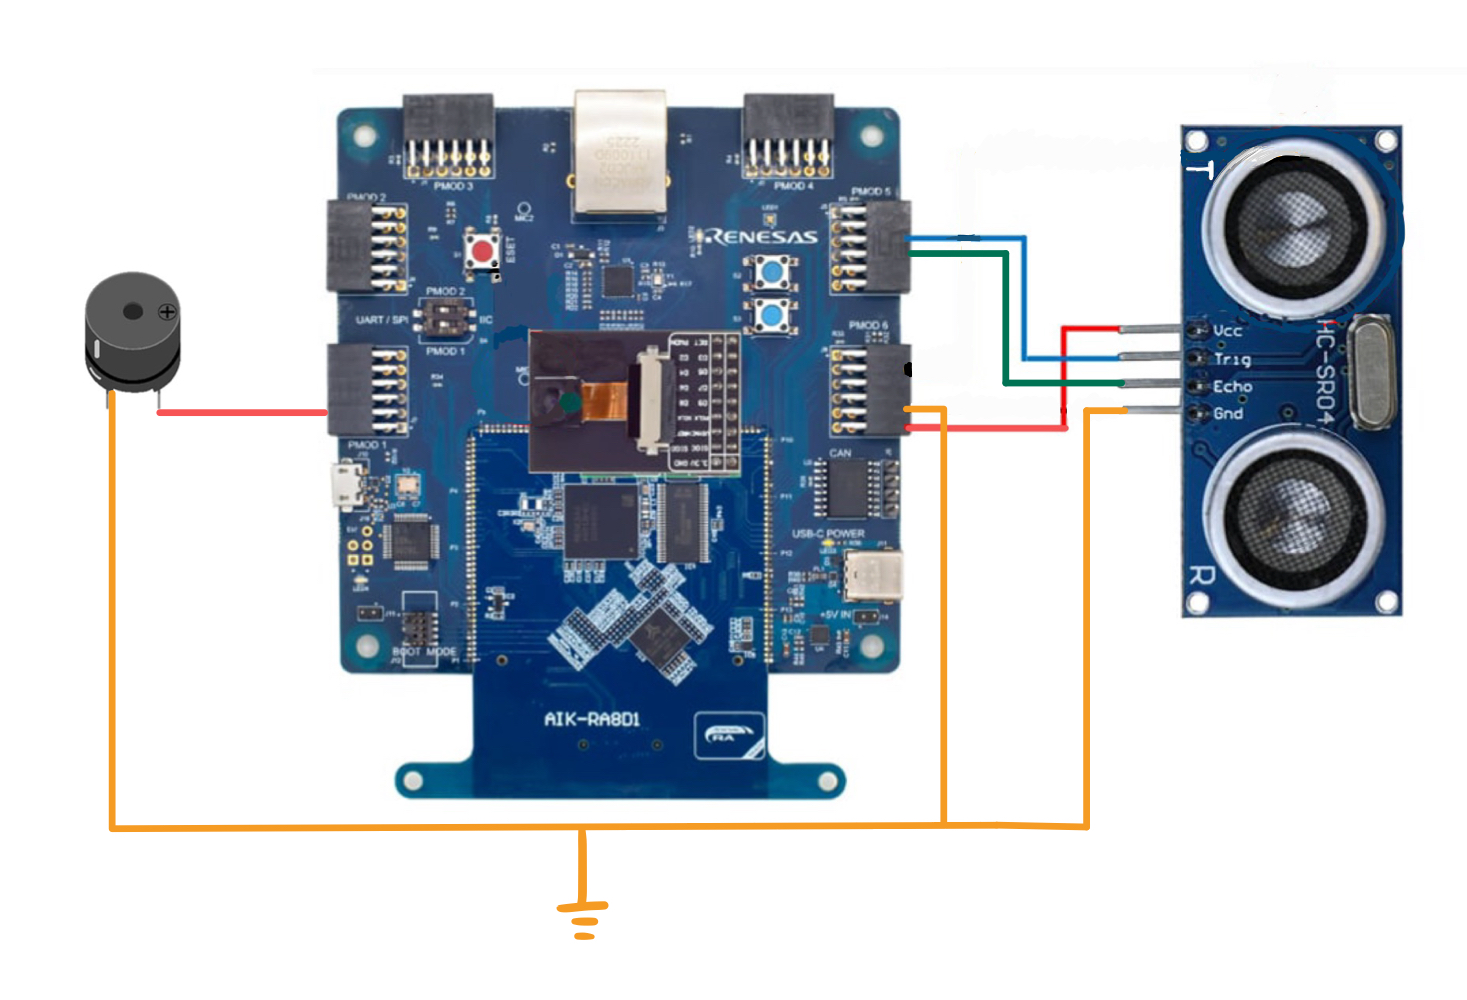
\includegraphics[width=0.85\columnwidth]{fig/circuit_schematic.jpg}
	\caption{hardware configurations}
\end{figure}
\begin{figure}[!h]
	\centering
	\subcaptionbox{Circuit deployment on our beloved AIK-RA8D1.
		\label{fig:reflector}}{
		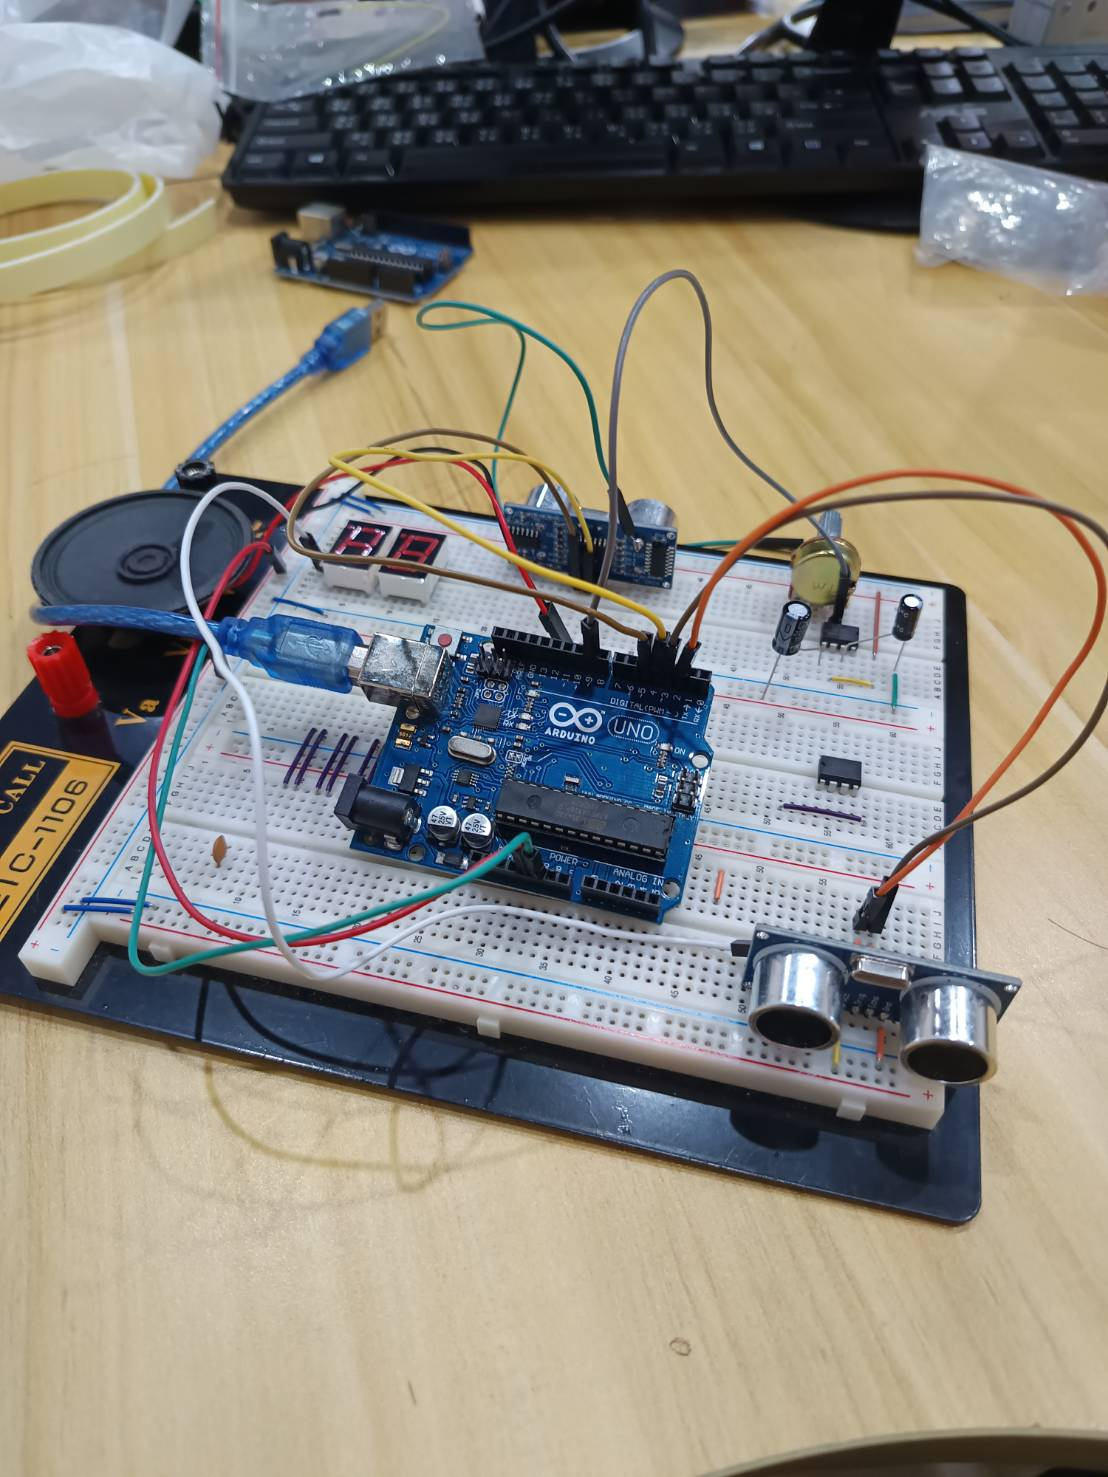
\includegraphics[height=0.45\columnwidth]{fig/arduino.jpg}}
	\subcaptionbox{measurement experiments setups. We use our tablet as the reflection board, and the distance is referenced with the table pad.
		\label{fig:stick_on_10k_board}}{
		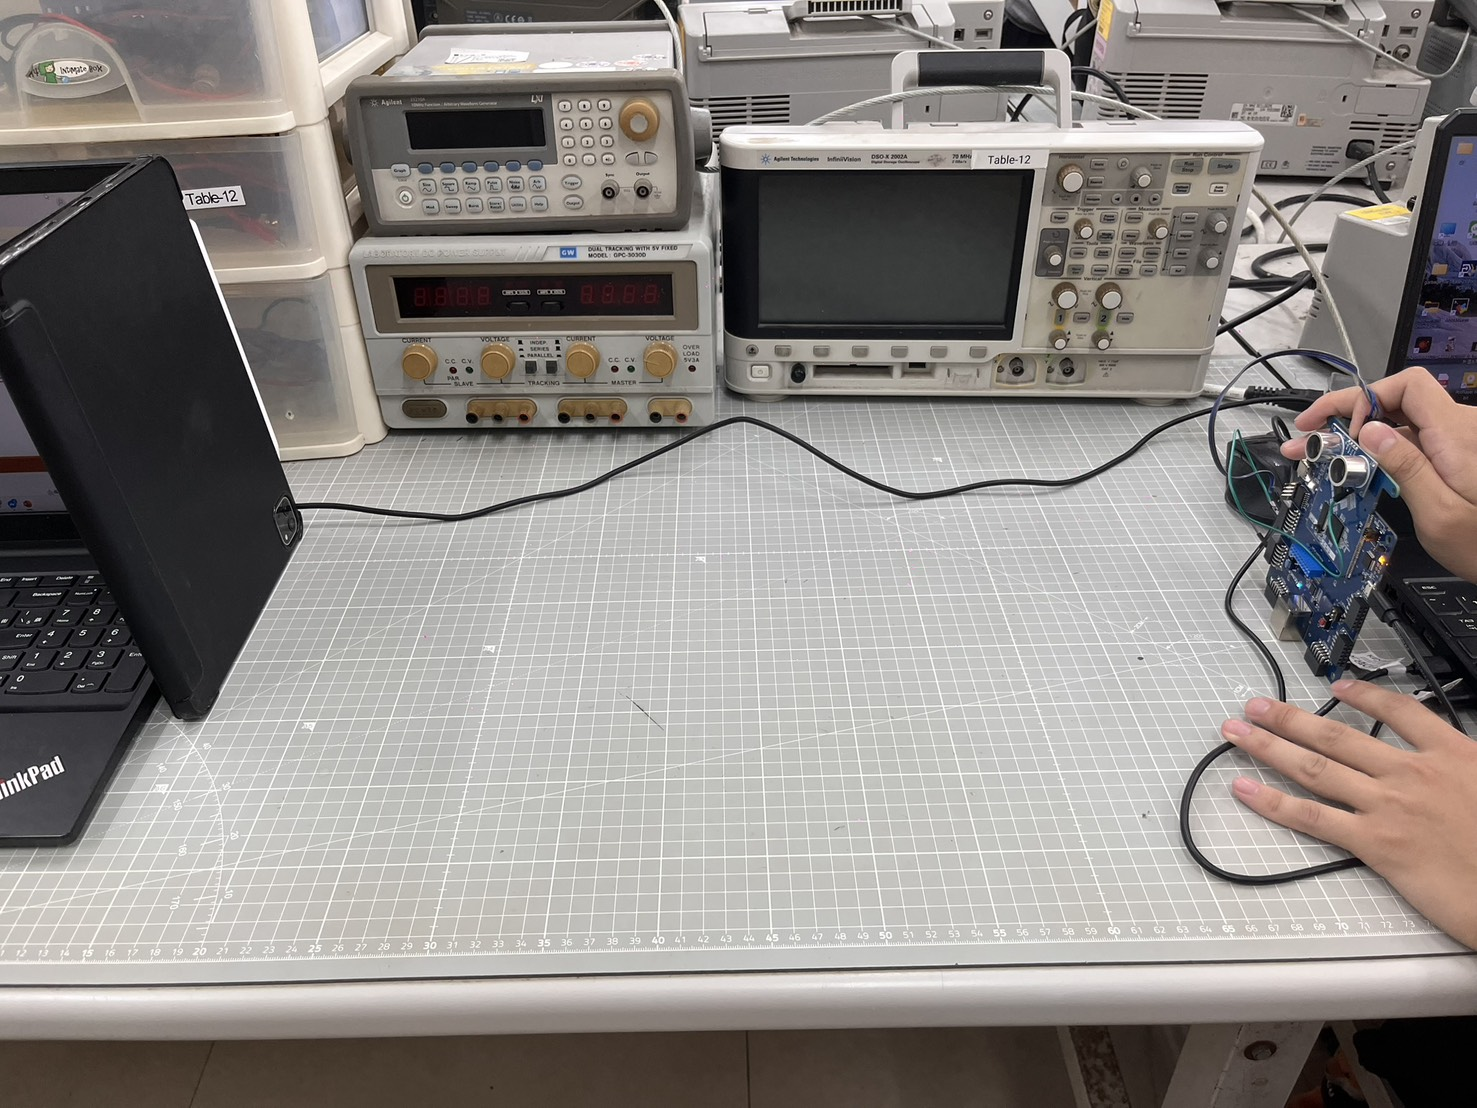
\includegraphics[height=0.45\columnwidth]{fig/S__59039761_0.jpg}}
	\caption{hardware configurations}
\label{fig:real_world_image}
\end{figure}

%%%%%%%%%%%%%%%%%%%%%%%%%%%%%%%%%%%%%%%%%%%%%%%%%%%%%%%%%%%%%%%%%%
\section{FPS configurations}
%%%%%%%%%%%%%%%%%%%%%%%%%%%%%%%%%%%%%%%%%%%%%%%%%%%%%%%%%%%%%%%%%%
To setup the MCU properly, we need to walk through a series of tracing. 
To start with, we need to first find the correct and compatible PIN that serves our desired purpose.
\subsection{PIN Hunting Procedure}

The following steps describe the systematic procedure used for PIN hunting:

\begin{enumerate}
    \item In the user manual documentation, identify the PIN that supports the desired function we need (e.g. P102). 
    \item In the Daughterboard schematic, locate the corresponding symbolic name (e.g., PMOD5\_SCK).
    \item Use this symbolic name to search for the signal in the Motherboard schematic.
    \item Check whether there are capacitors, resistors, or other components on the signal path that may affect signal integrity in the schematic.
    \item Record the exact numbering on the board (e.g., J5-4).
    \item Locate the correct physical pin on the actual hardware board.
    \item Set up the hardware accordingly.
\end{enumerate}

\begin{figure}[!h]
	\centering
	\subcaptionbox{ Daughterboard Schematic, where we can find how the PIN correspond to the symbolic name in the Motherboard Schematic.
		\label{fig:daughter_schematic}}{
		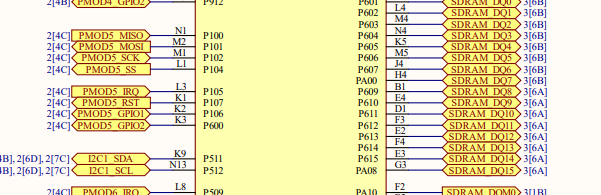
\includegraphics[width=0.45\columnwidth]{fig/daughter_sch.png}}
	\subcaptionbox{ Use the identified symbolic name to find the exact location on the board.
		\label{fig:mother_schematic}}{
		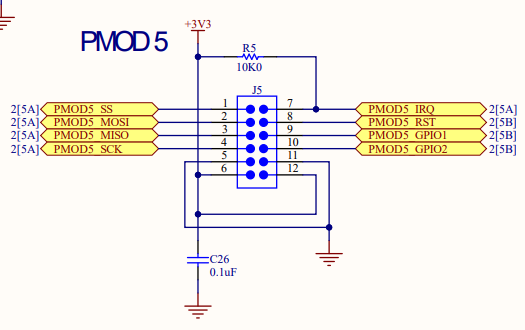
\includegraphics[width=0.45\columnwidth]{fig/mother_sch.png}}

	\caption{hardware configurations}
\label{fig:pin_schematic_hunt}
\end{figure}


\subsection{FSP configuration}
Since one single PIN usually support multiple functions, in the $e^2$ studio we need to set each of them to the actual function we expect them to work.
\begin{enumerate}
    \item In the FSP Configuration tool, under the \texttt{Pins} tab, locate the desired PIN in the \texttt{Ports} list.
    \item Check the capability of the selected port and configure it to the appropriate function.
    \item If the PIN is already occupied, navigate to the \texttt{Peripherals} section and disconnect the original function.
    \item Ensure that the original function is not required before reassignment.
\end{enumerate}

\begin{figure}[!h]
	\centering
	\subcaptionbox{ FSP Peripherals tab. 
		\label{fig:FSP_pin}}{
		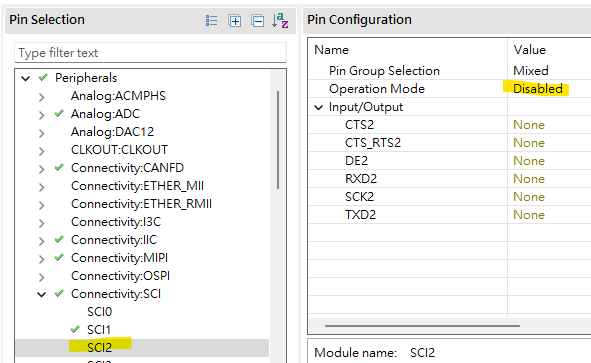
\includegraphics[width=0.45\columnwidth]{fig/FPS_peripheral.png}}
	\subcaptionbox{ FSP Pins tab. 
		\label{fig:FSP_peripherals}}{
		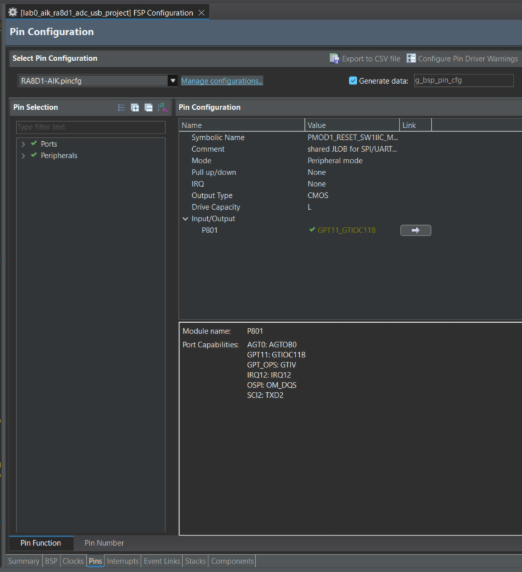
\includegraphics[width=0.45\columnwidth]{fig/FPS_pin_config.png}}
	\caption{FSP configurations}
\label{fig:FSP_configuration}
\end{figure}

%%%%%%%%%%%%%%%%%%%%%%%%%%%%%%%%%%%%%%%%%%%%%%%%%%%%%%%%%%%%%%%%%%
\section{HC-SR04--Distance Measurement Module}
%%%%%%%%%%%%%%%%%%%%%%%%%%%%%%%%%%%%%%%%%%%%%%%%%%%%%%%%%%%%%%%%%%

\subsection{Trigger Pin Configuration and Signal Specification}
\label{subsec:trigger_pin}

The trigger signal is generated by the MCU to provide a periodic TTL-level timing reference for external modules. This subsection describes the hardware configuration, timing source, and electrical and temporal specifications of the trigger pin.

\subsubsection{Pin Assignment}

The trigger output is assigned to pin \texttt{P100}.  
This pin is configured as a GPIO output under the Renesas Flexible Software Package (FSP) pin configuration interface.

\begin{itemize}
    \item \textbf{Pin}: \texttt{P100}
    \item \textbf{Direction}: Output
    \item \textbf{Output type}: CMOS
    \item \textbf{Logic level}: TTL-compatible
\end{itemize}

The output polarity is configured as \emph{initial low}, and the pin is driven directly by the timer output logic without additional hardware gating.

\subsubsection{Timer Source: Asynchronous General Timer (AGT)}

The trigger signal is generated using the AGT, a low-power timer peripheral designed to operate independently of the high-speed system clock. It is suitable for periodic signal generation with minimal power consumption.

\begin{itemize}
    \item \textbf{Timer module}: AGT
    \item \textbf{Channel}: 0
    \item \textbf{Counter width}: 16-bit
    \item \textbf{Maximum count value}: $2^{16} = 65536$
\end{itemize}


\subsubsection{Clock Source and Timing Resolution}

The AGT is driven by a low-power clock source.  
This clock determines the fundamental timing resolution of the trigger signal.

\begin{itemize}
    \item \textbf{Clock type}: Low-power clock
    \item \textbf{Effective clock frequency}: Set to $27~\text{kHz}$ in FSP
\end{itemize}

All timing parameters (pulse width and period) are derived from this clock frequency.

\subsubsection{Trigger Signal Timing Specification}

The trigger pin outputs a periodic TTL pulse with the following characteristics:

\begin{itemize}
    \item \textbf{Pulse width}: $10~\mu\text{s}$
    \item \textbf{Repetition rate}: approximately $26.67~\text{kHz}$
\end{itemize}

The pulse width is defined by the AGT compare match value, while the period is defined by the timer overflow value.

A timing diagram of the trigger signal is illustrated conceptually as:

\begin{center}
\texttt{HIGH (10~$\mu$s)} $\rightarrow$ \texttt{LOW} $\rightarrow$ repeat
\end{center}

\begin{figure}[H]
	\centering
		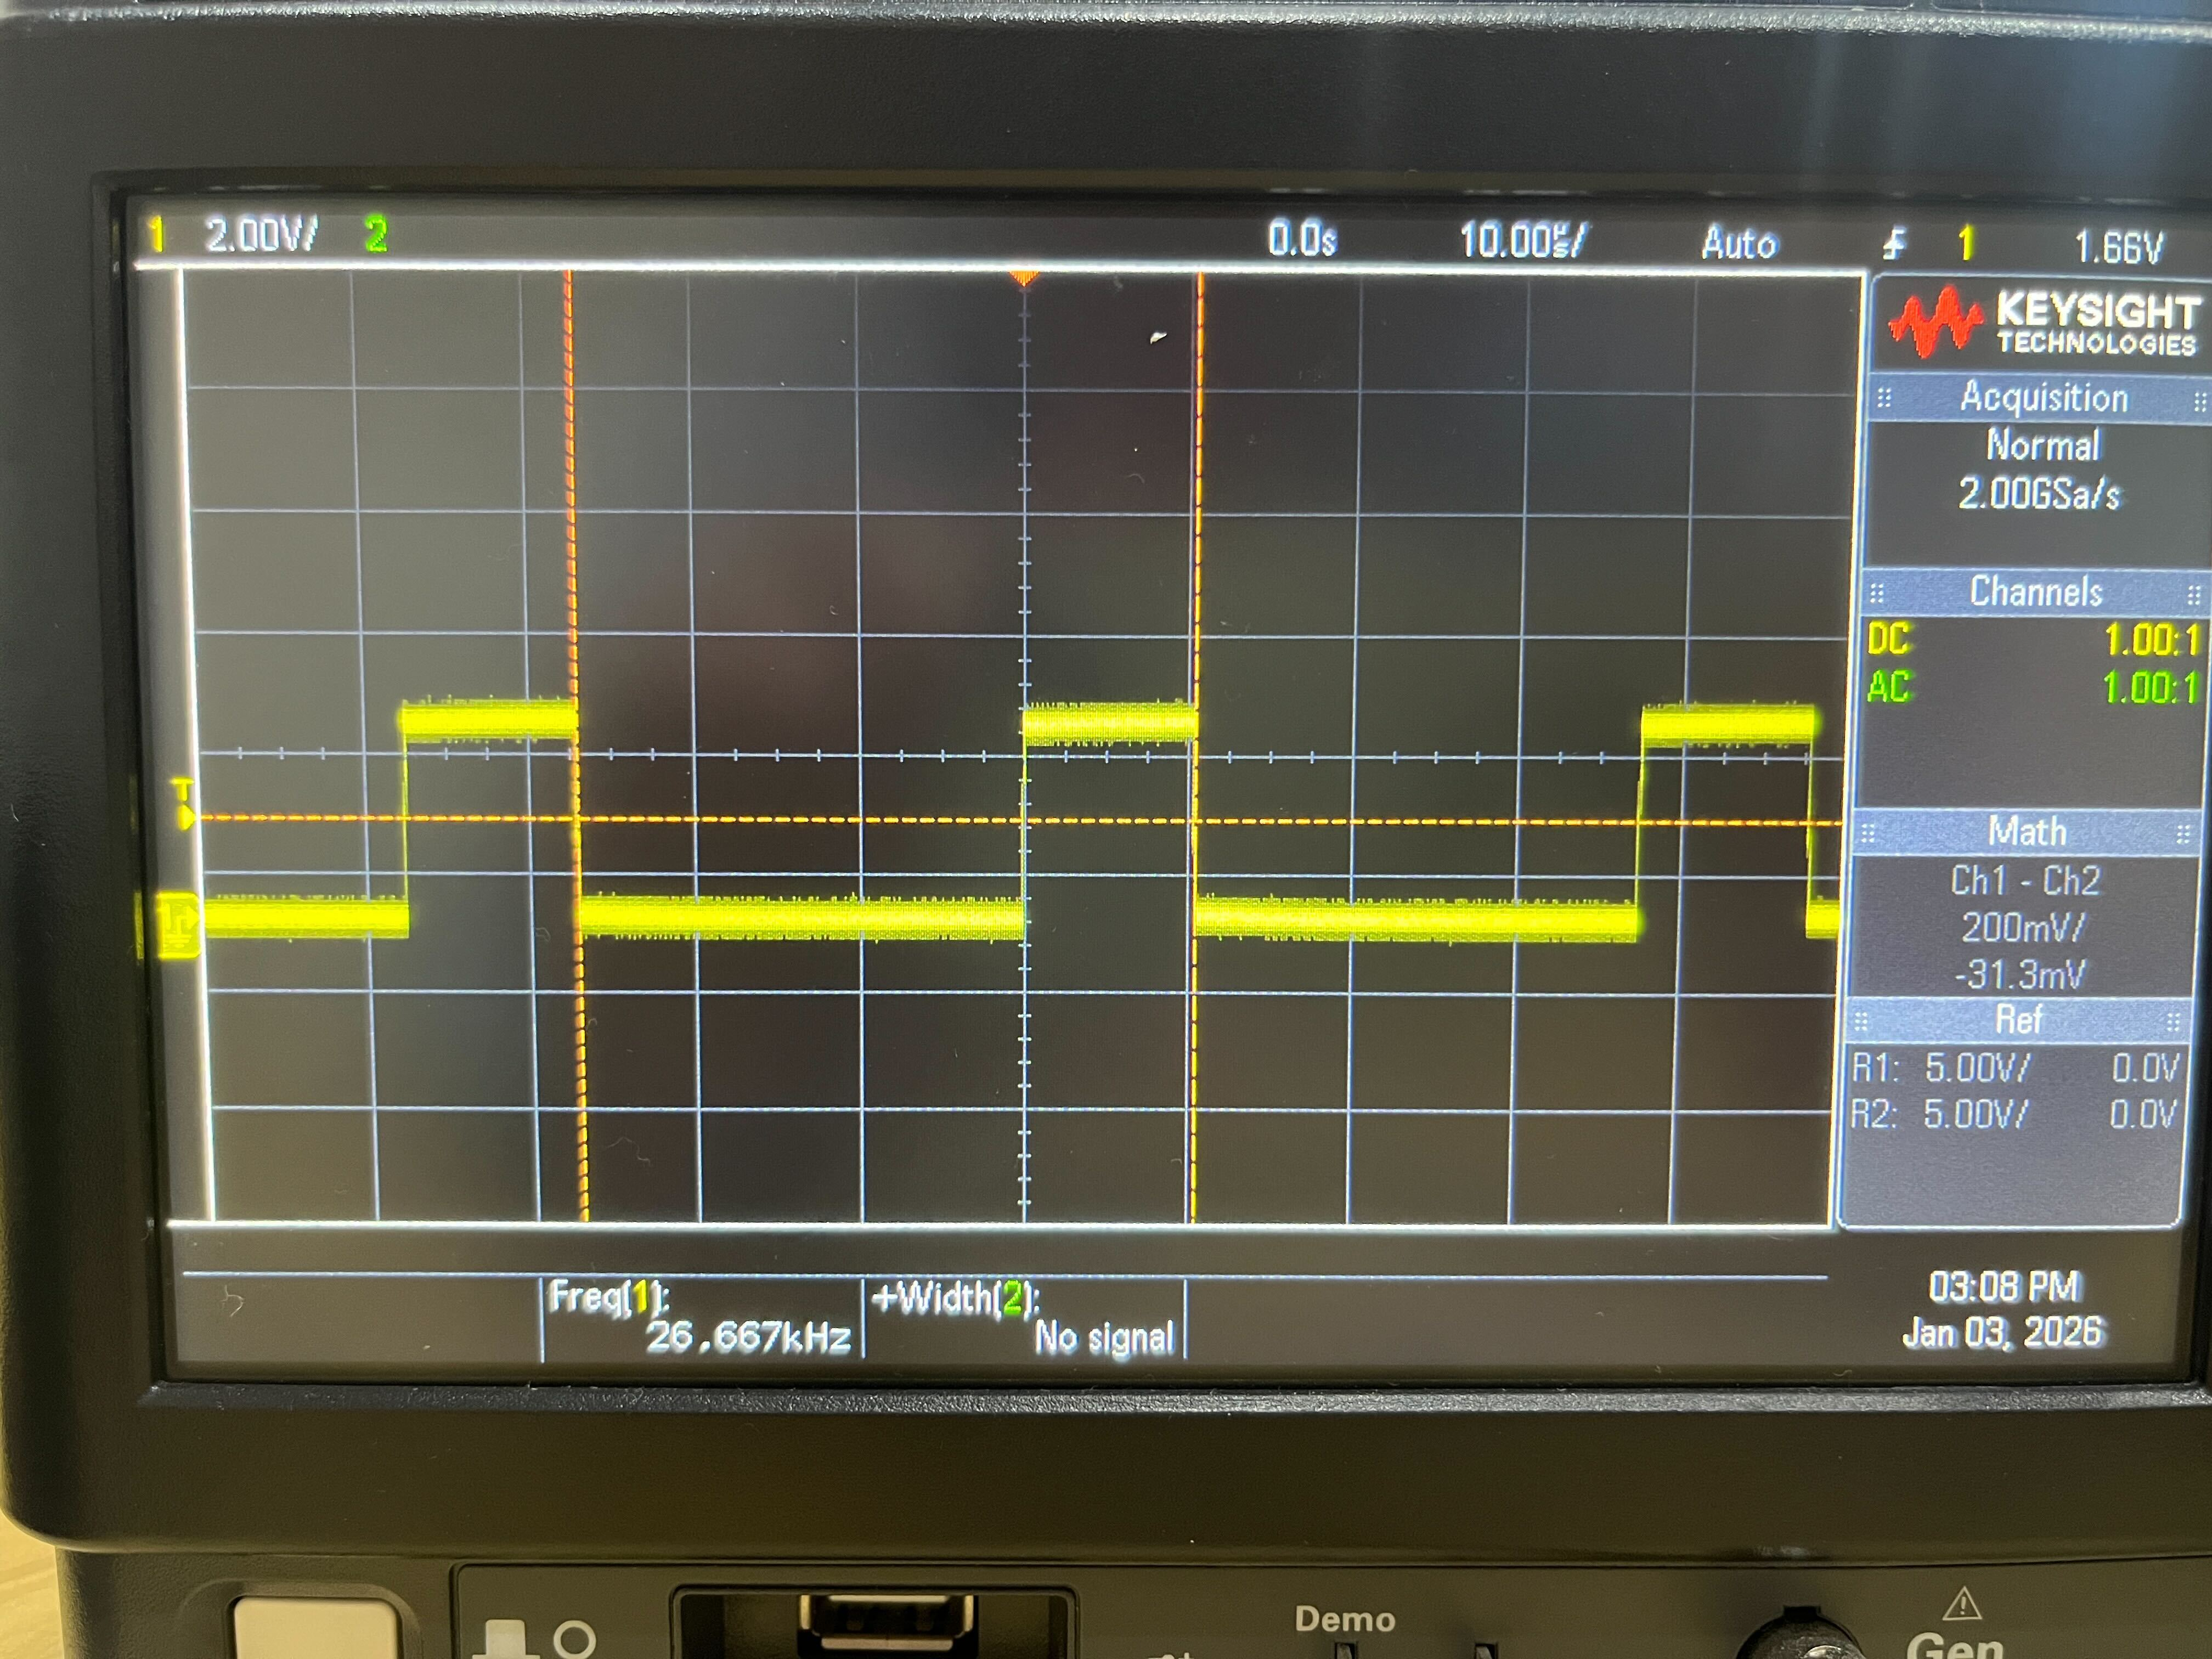
\includegraphics[width=0.65\columnwidth]{fig/trigger_pin_signal.jpg}
	\caption{The signal Output by P100. This is served as the input signal to the Trigger pin. We can see that }
\label{fig:trigger_pin_osc}
\end{figure}

\subsection{Echo Pin Configuration and Measurement Principle}
\label{subsec:echo_pin}

The echo pin is used to receive a TTL-level pulse whose duration encodes the round-trip propagation time of the transmitted signal. This subsection describes the timer configuration, edge detection strategy, and distance computation method.

\subsubsection{Pin and Timer Assignment}

The echo signal is connected to pin \texttt{P102}, which is configured as a timer input channel.

\begin{itemize}
    \item \textbf{Pin}: \texttt{P102}
    \item \textbf{Timer module}: General PWM Timer (GPT)
    \item \textbf{Channel}: GPT2, GTIO Channel 2B
    \item \textbf{Mode}: Periodic
    \item \textbf{Counter width}: 16-bit
    \item \textbf{Period}: \texttt{0x10000} (raw counts)
\end{itemize}

The GPT counter runs continuously and provides a free-running time base for pulse width measurement.

\subsubsection{Edge Detection and Time Measurement}

To measure the pulse width of the echo signal, both edges of the input waveform are detected:

\begin{itemize}
    \item \textbf{Rising edge}: marks the start of the echo pulse
    \item \textbf{Falling edge}: marks the end of the echo pulse
\end{itemize}

The timer count values are captured at each edge. The difference between the captured counts corresponds to the pulse duration in timer ticks.

\subsubsection{Echo Pulse Interpretation}

The echo pin receives a TTL-level pulse whose high-level duration is proportional to the signal’s round-trip time of flight. Conceptually,

\begin{center}
\texttt{Pulse Width} $\;\propto\;$ \texttt{Propagation Time}
\end{center}

This pulse is generated by the external module and fed directly into the GPT input capture logic.

\subsubsection{Distance Conversion}

Let $x$ denote the measured pulse width in microseconds. The corresponding distance is computed as

\[
\text{Distance (cm)} = \frac{x}{58}
\]

This conversion factor accounts for the round-trip travel time of the signal and the propagation speed in air.

\subsubsection{Functional Role of the Echo Pin}

The echo pin serves as the timing measurement input that:
\begin{itemize}
    \item captures the duration of the returned signal,
    \item enables distance estimation based on time-of-flight,
    \item operates independently of the trigger generation logic.
\end{itemize}

Using GPT input capture ensures accurate edge-aligned timing measurement with minimal software overhead.

\begin{figure}[H]
	\centering
	\caption{The signal Output by echo pin. The green curve is the PWM signal carrying the ToF with distance $d = 5cm$, and the yellow curve is the trigger pin signal. This in} 
\label{fig:echo_pin_signal}
\end{figure}

\begin{figure}[!h]
	\centering
	\subcaptionbox{ 15cm. ToF $=941.8 \mu s$ 
		\label{fig:echo_5cm}}{
		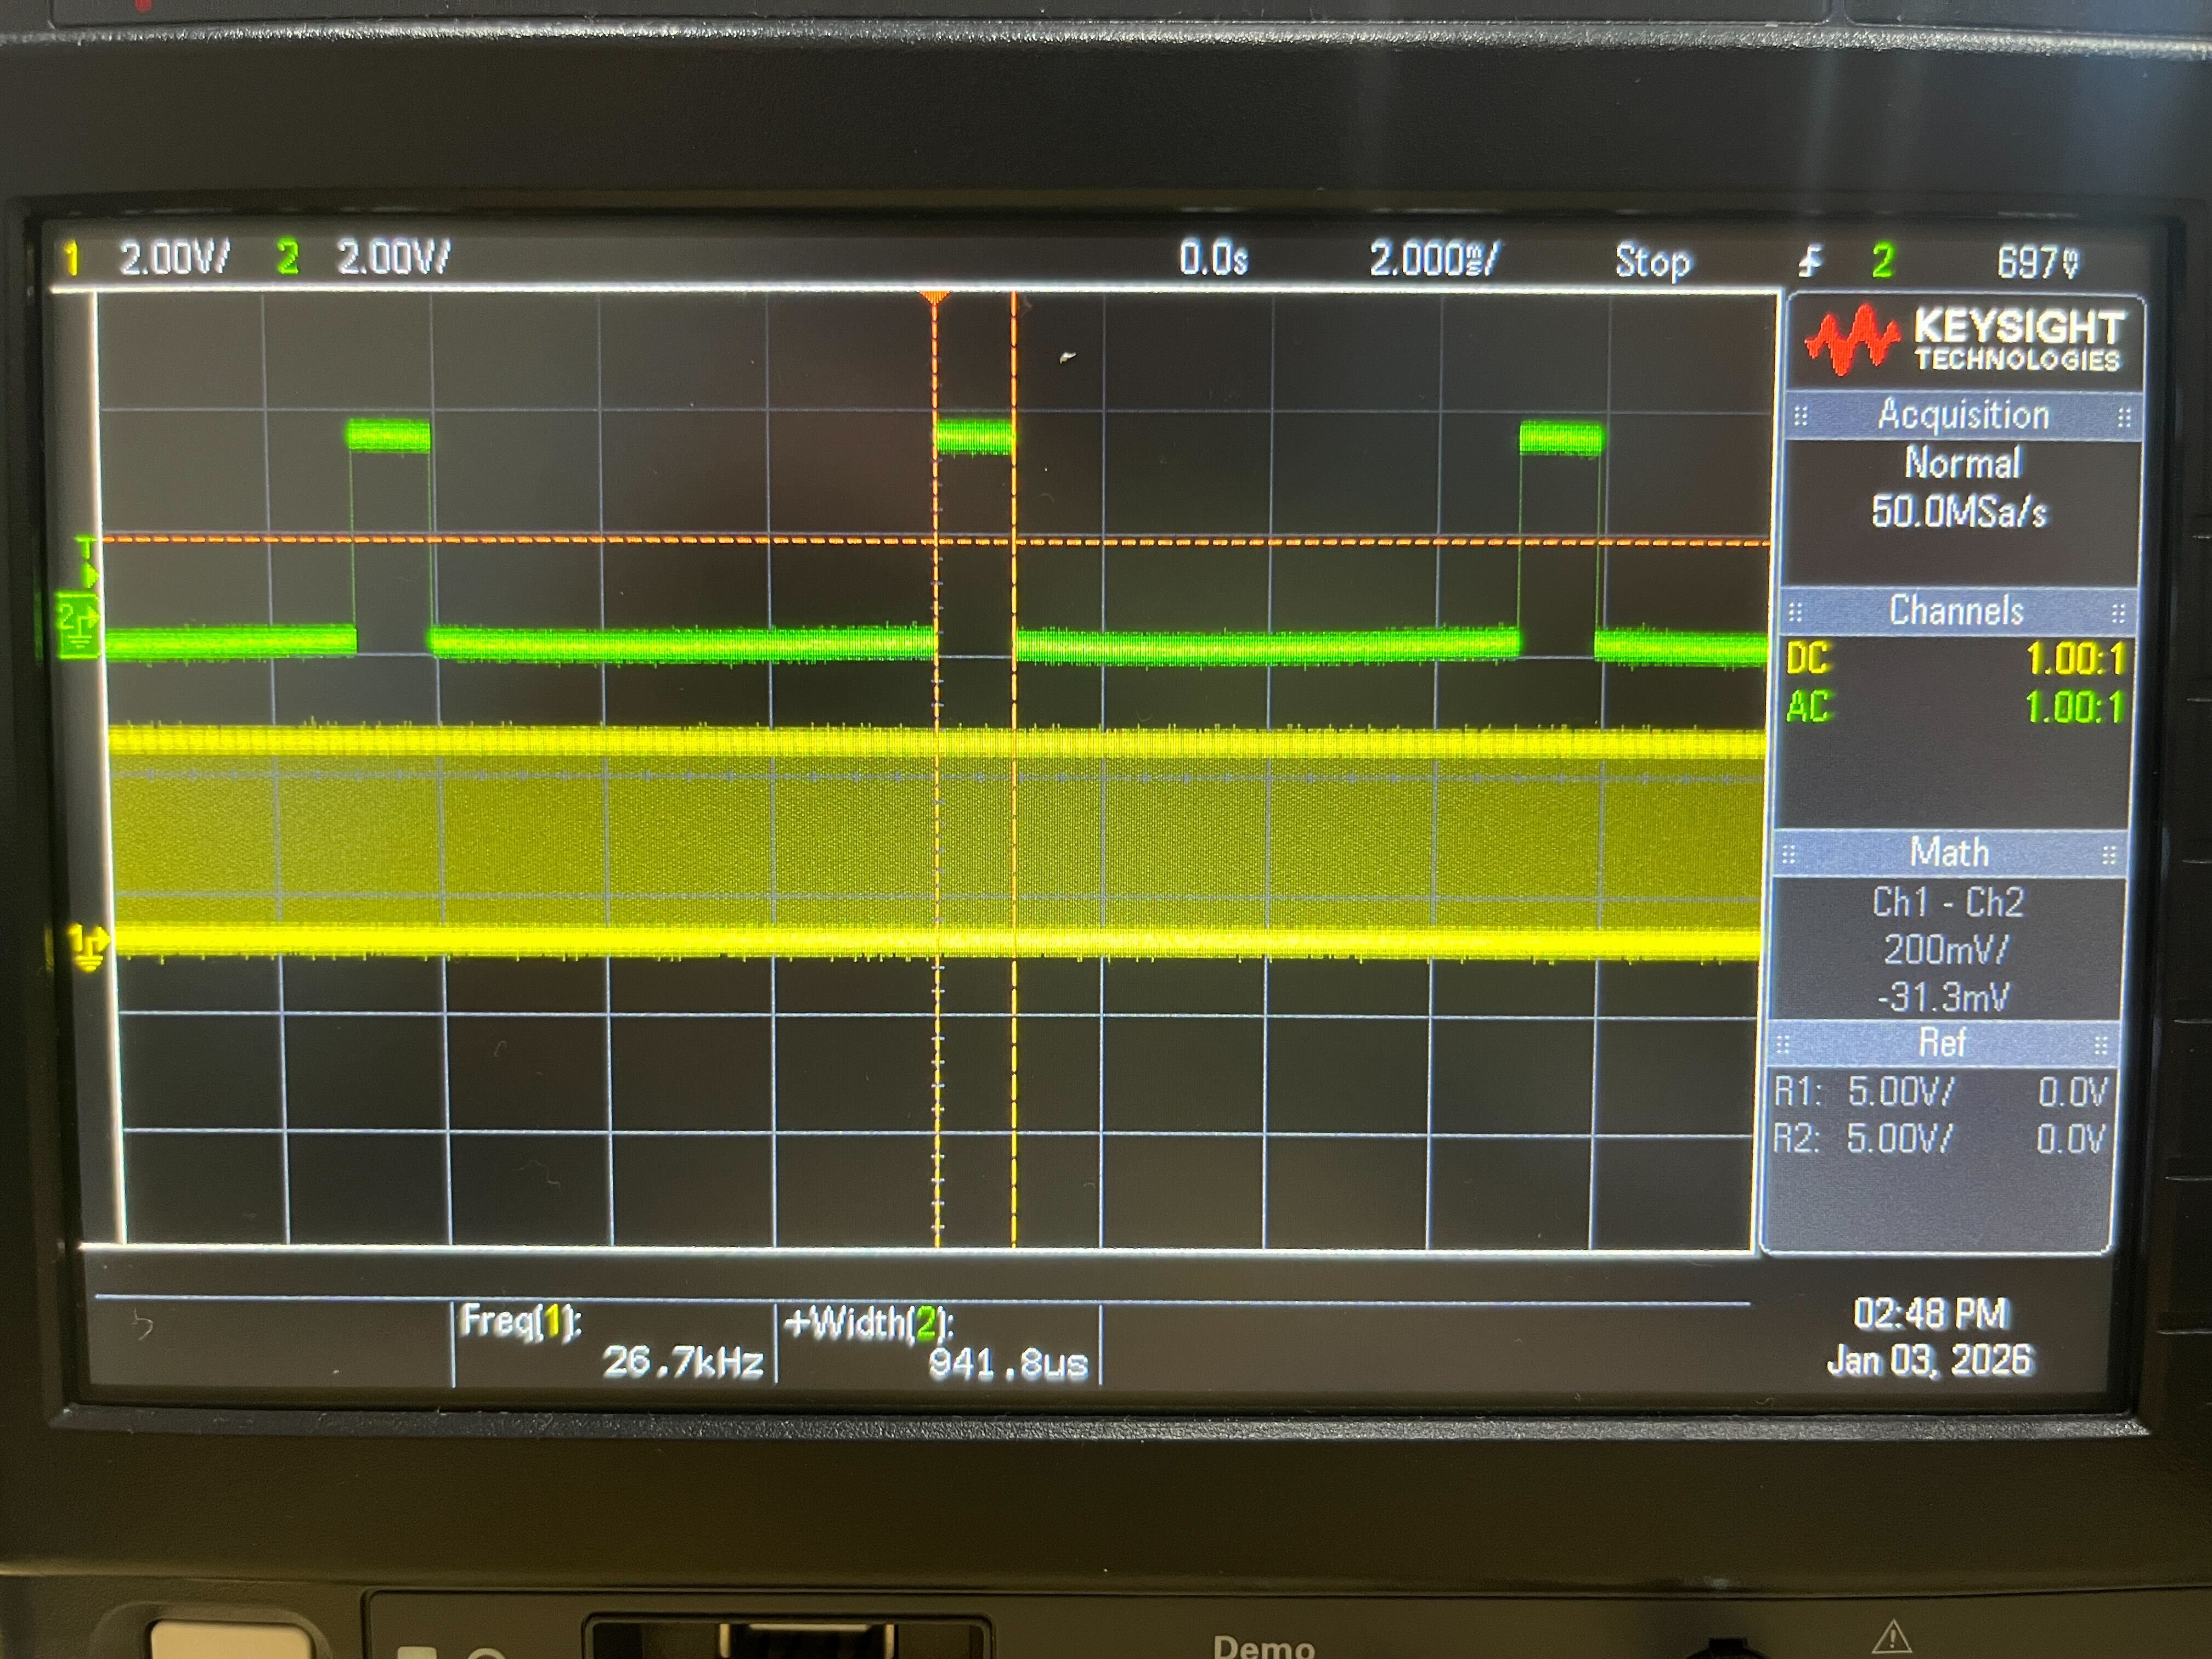
\includegraphics[width=0.45\columnwidth]{fig/echo_only_5.jpg}}
	\subcaptionbox{ 30cm. ToF $=1848.6 \mu s$ 
		\label{fig:echo_10cm}}{
		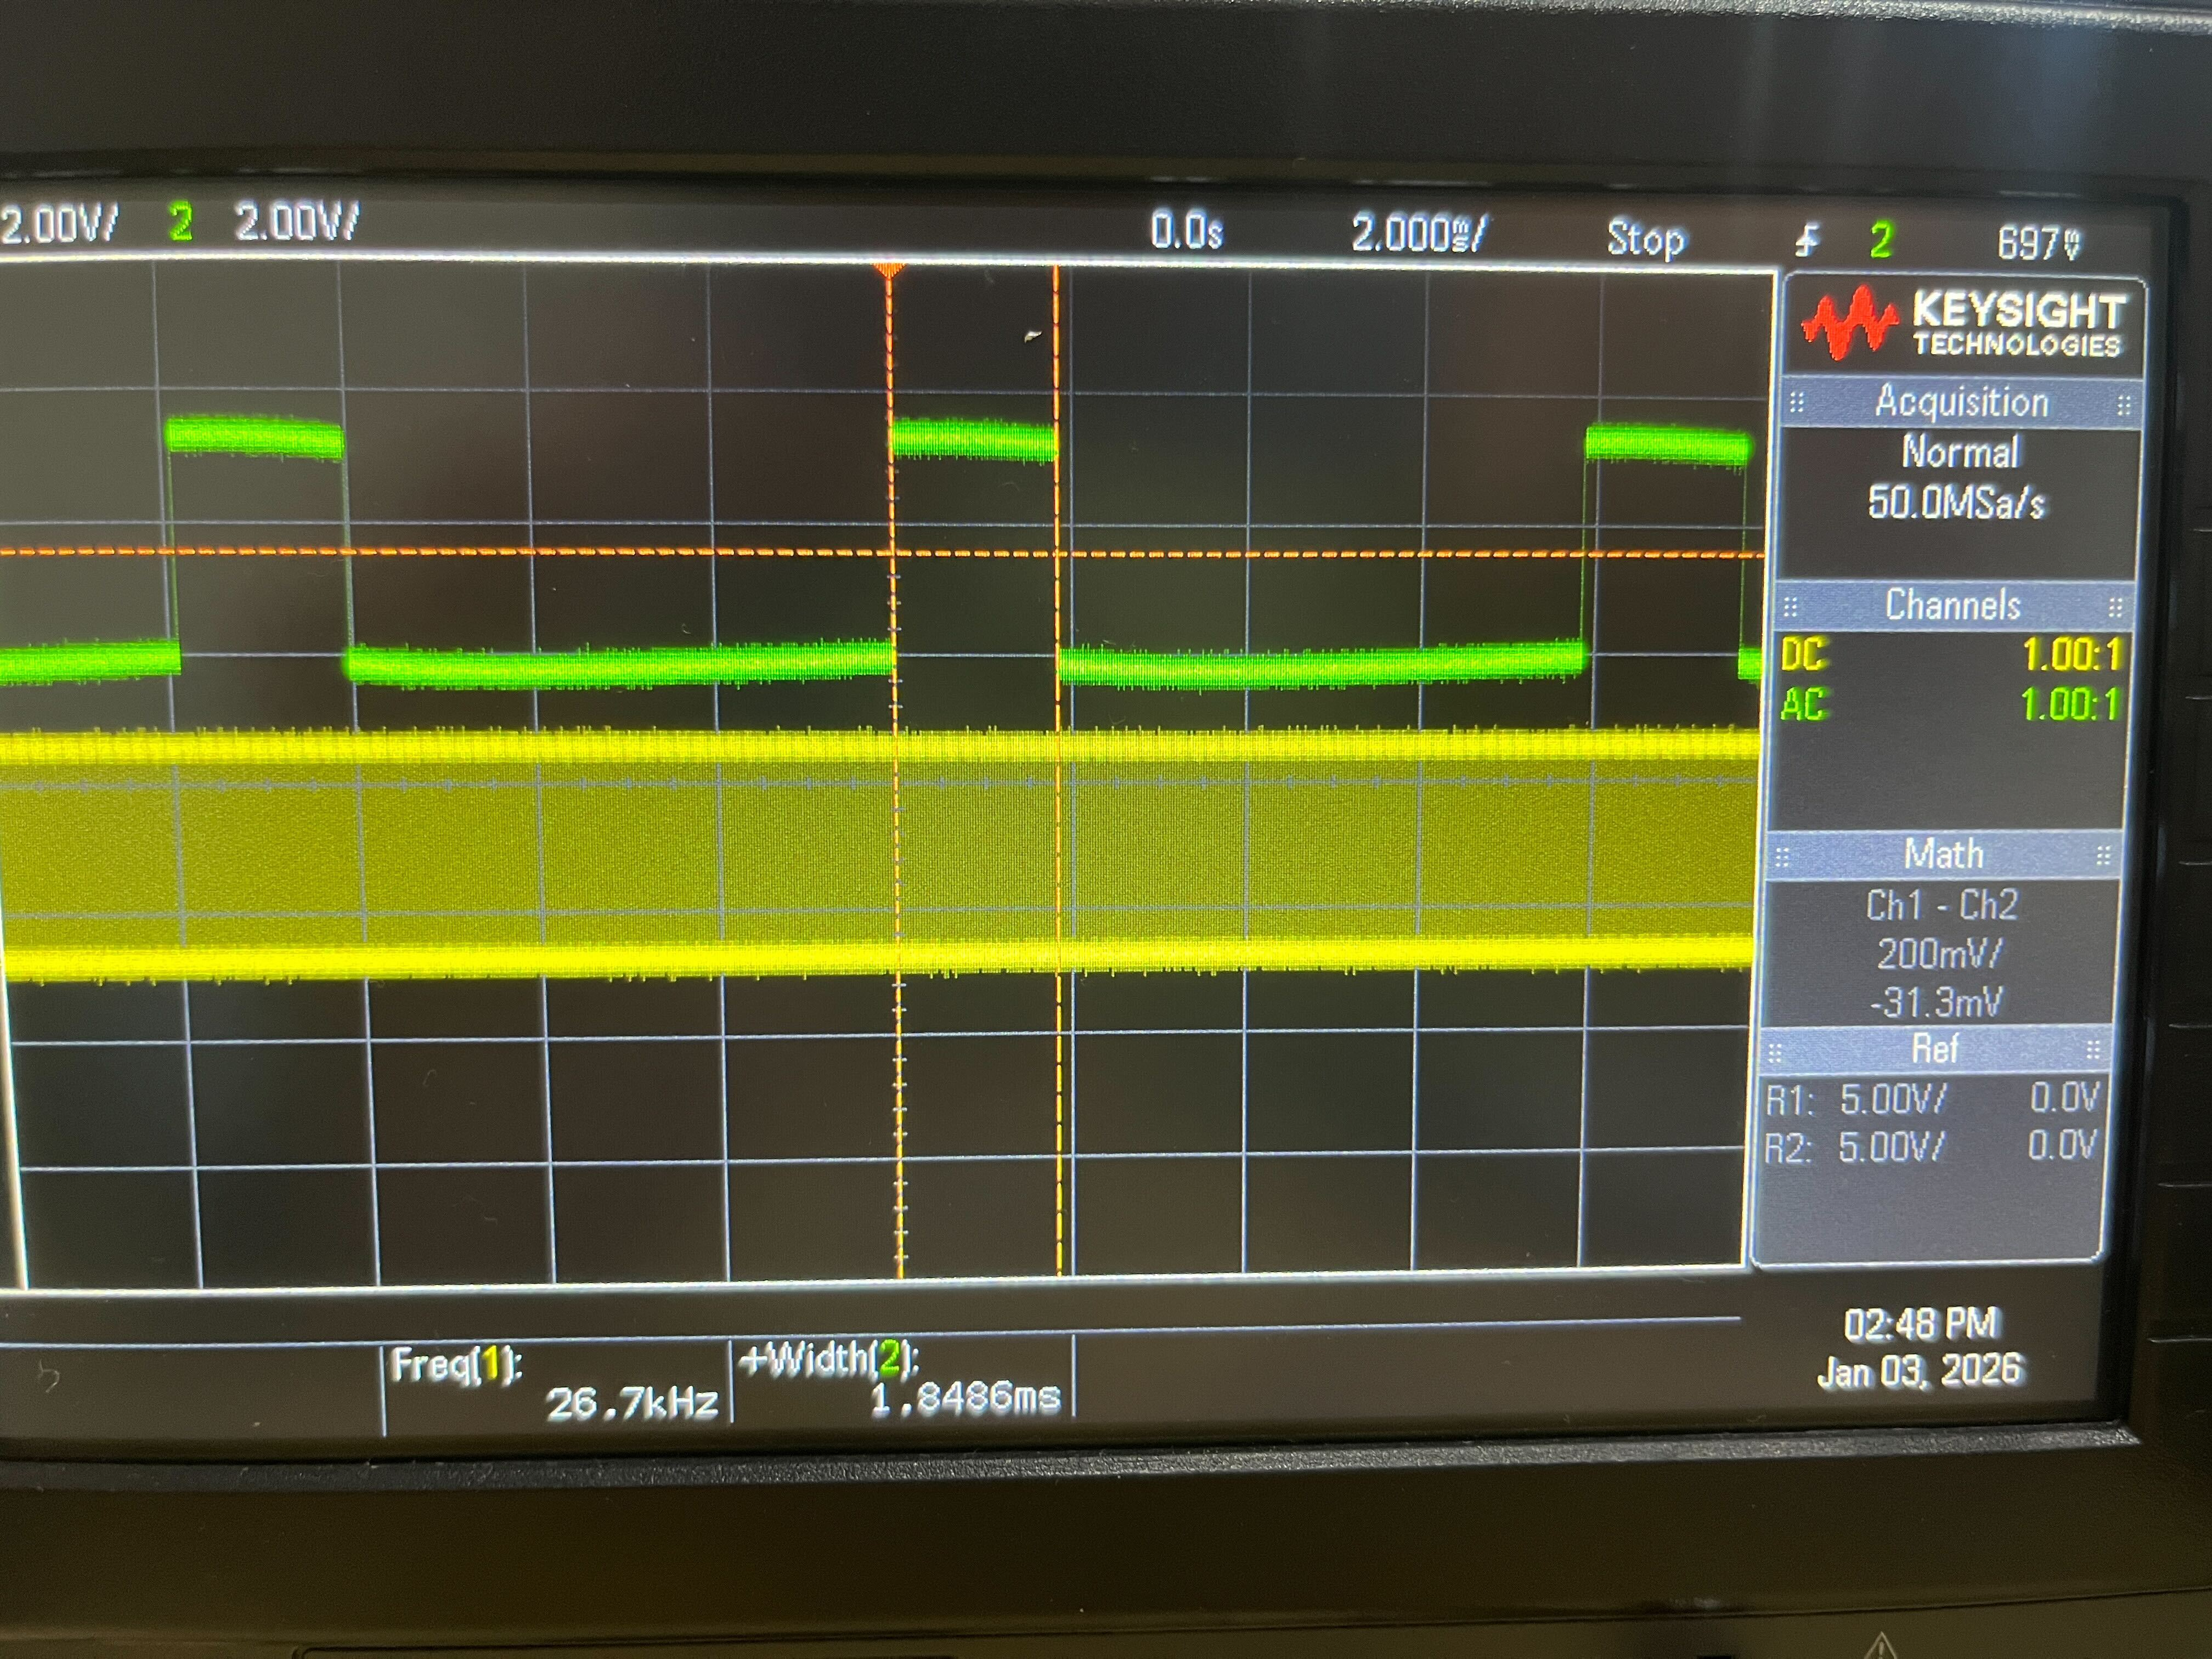
\includegraphics[width=0.45\columnwidth]{fig/echo_only_30.jpg}}
	\caption{Echo Pin output signal with different distance. The green wave is the square pulse sent by echo pin, and the yellow wave is the trigger pin signal. 
  This indicates that the Module is functioning as expected, all the configuration has been properly set.}
\label{fig:echo_dist}
\end{figure}

\subsubsection{Callback Function}

We are now able to finally implement how we want our board to react once they've detected the expected rising/falling signal from the echo pin, and convert it back to distance.

\begin{figure}[H]
\centering
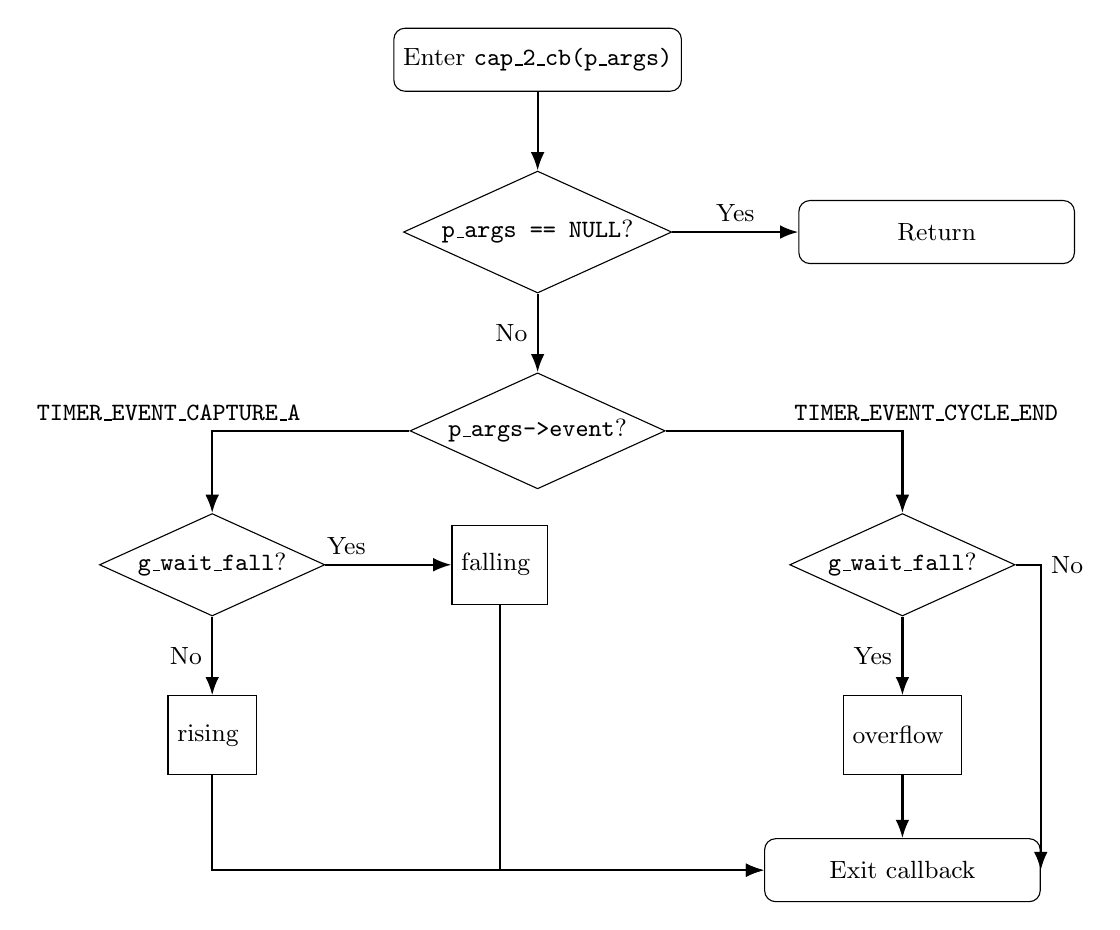
\begin{tikzpicture}[
    node distance=10mm and 16mm,
    font=\small,
    startstop/.style={rectangle, rounded corners, draw, align=center, minimum width=35mm, minimum height=8mm},
    process/.style={rectangle, draw, align=left, minimum width=10mm, minimum height=10mm},
    decision/.style={diamond, draw, align=center, aspect=2.2, inner sep=1.5pt},
    connector/.style={circle, draw, minimum size=5mm, inner sep=0pt},
    arrow/.style={-Latex, thick}
]
% --- Nodes ---
\node[startstop] (entry) {Enter \texttt{cap\_2\_cb(p\_args)}};
\node[decision, below=of entry] (nullcheck) {\texttt{p\_args == NULL}?};
\node[startstop, right=of nullcheck] (ret) {Return};
\node[decision, below=of nullcheck] (event) {\texttt{p\_args->event}?};

% --- Capture A branch ---
\node[decision, below left=of event, xshift=-10mm] (waitfall) {\texttt{g\_wait\_fall}?};
\node[process, below=of waitfall] (rise) {
rising
};
\node[process, right=of waitfall] (fall) {
 falling
};

% --- Cycle end branch ---
\node[decision, below right=of event, xshift=15mm] (cyclewait) {\texttt{g\_wait\_fall}?};
\node[process, below=of cyclewait] (overflow) {
  overflow
};

% --- Default / exit ---
\node[startstop, below=8mm of overflow] (exit) {Exit callback};

% --- Arrows ---
\draw[arrow] (entry) -- (nullcheck);
\draw[arrow] (nullcheck) -- node[above]{Yes} (ret);
\draw[arrow] (nullcheck) -- node[left]{No} (event);

% Switch branches
\draw[arrow] (event) -| node[near start, above left]{\texttt{TIMER\_EVENT\_CAPTURE\_A}} (waitfall);
\draw[arrow] (event) -| node[near start, above right]{\texttt{TIMER\_EVENT\_CYCLE\_END}} (cyclewait);

% Capture A: edge-state machine
\draw[arrow] (waitfall) -- node[left]{No} (rise);
\draw[arrow] (waitfall) -- ++(25mm,0) node[above, near start]{Yes} |- (fall);
\draw[arrow] (rise) |- (exit);
\draw[arrow] (fall) |- (exit);

% Cycle end: overflow counting only when waiting for falling edge
\draw[arrow] (cyclewait) -- node[left]{Yes} (overflow);
\draw[arrow] (cyclewait.east) -| node[right]{No} (exit.east);
% \draw[arrow] (cyclewait.south) -- ++(0,-8mm) node[right, near start]{No} -| (exit.north);
\draw[arrow] (overflow) -- (exit);

\end{tikzpicture}
\caption{Control flow of the GPT2 input-capture callback for echo pulse measurement.}
\label{fig:gpt2_callback_flow}
\end{figure}



\begin{lstlisting}[language=C, caption={GPT2 Input Capture Callback for Echo Pulse Measurement}, label={lst:gpt2_callback}]
void cap_2_cb(timer_callback_args_t *p_args)
{
    if (NULL == p_args)
    {
        return;
    }

    switch (p_args->event)
    {
        case TIMER_EVENT_CAPTURE_A:
        {
            if (!g_wait_fall)
            {
                /* First edge: treat as rising */
                g_echo_rise = (uint32_t) p_args->capture;
                g_capture_overflow = 0;
                g_wait_fall = true;
            }
            else
            {
                /* Second edge: treat as falling */
                g_echo_fall = (uint32_t) p_args->capture;
                g_wait_fall = false;
                b_start_measurement = true;
            }
            break;
        }

        case TIMER_EVENT_CYCLE_END:
        {
            /* Timer wrapped between rise and fall */
            if (g_wait_fall)
            {
                g_capture_overflow++;
            }
            break;
        }

        default:
            break;
    }
}
\end{lstlisting}

%%%%%%%%%%%%%%%%%%%%%%%%%%%%%%%%%%%%%%%%%%%%%%%%%%%%%%%%%%%%%%%%%%
\section{HPE-122 Passive Buzzer}
%%%%%%%%%%%%%%%%%%%%%%%%%%%%%%%%%%%%%%%%%%%%%%%%%%%%%%%%%%%%%%%%%%
\label{subsec:buzzer}

We choose a cheap passive buzzer as our audio output module since we are familiar with it.

\subsection{FPS configuration}
The buzzer is driven by a hardware PWM signal generated using the General PWM Timer (GPT). This subsection describes the pin assignment, timer configuration, and achievable output frequency range.

\subsubsection{Pin and Timer Assignment}

The buzzer output is mapped to pin \texttt{P801}, which is configured as a GPT output channel.

\begin{itemize}
    \item \textbf{Pin}: \texttt{P801}
    \item \textbf{Timer module}: GPT
    \item \textbf{Channel}: GPT11
    \item \textbf{Output channel}: GTIO Channel 11B
\end{itemize}


\subsubsection{PWM Configuration}

The GPT is configured in saw-wave PWM mode to generate a square-wave signal suitable for driving a buzzer.

\begin{itemize}
    \item \textbf{PWM mode}: Saw-wave PWM
    \item \textbf{Output channel enabled}: Channel B
    \item \textbf{Duty cycle}: 50\%
    \item \textbf{Initial output level}: Low
\end{itemize}

Channel~A output is disabled, and only Channel~B is used to simplify signal routing.

\subsubsection{Operating Frequency}

The PWM output frequency is set to approximately $1~\text{kHz}$, which lies within the audible range and is appropriate for buzzer operation.

\subsubsection{Allowed Output Frequency Range}

The GPT operates with the following constraints:

\begin{itemize}
    \item \textbf{Clock frequency}: $60~\text{MHz}$
    \item \textbf{Counter width}: 16-bit
\end{itemize}

The minimum achievable output frequency is therefore limited by the maximum counter period:

\[
f_{\min} = \frac{60~\text{MHz}}{2^{16}} \approx 915~\text{Hz}
\]

The actual timer parameters and clock frequency are verified at runtime using \texttt{R\_GPT\_InfoGet}.

\subsubsection{Functional Role}

The buzzer signal provides audible feedback to the user. Its frequency and duty cycle are controlled entirely in hardware, ensuring stable operation with minimal CPU involvement.

\begin{figure}[!h]
	\centering
	\subcaptionbox{ 10cm, 1.2598kHz 
		\label{fig:buzzer_10cm}}{
		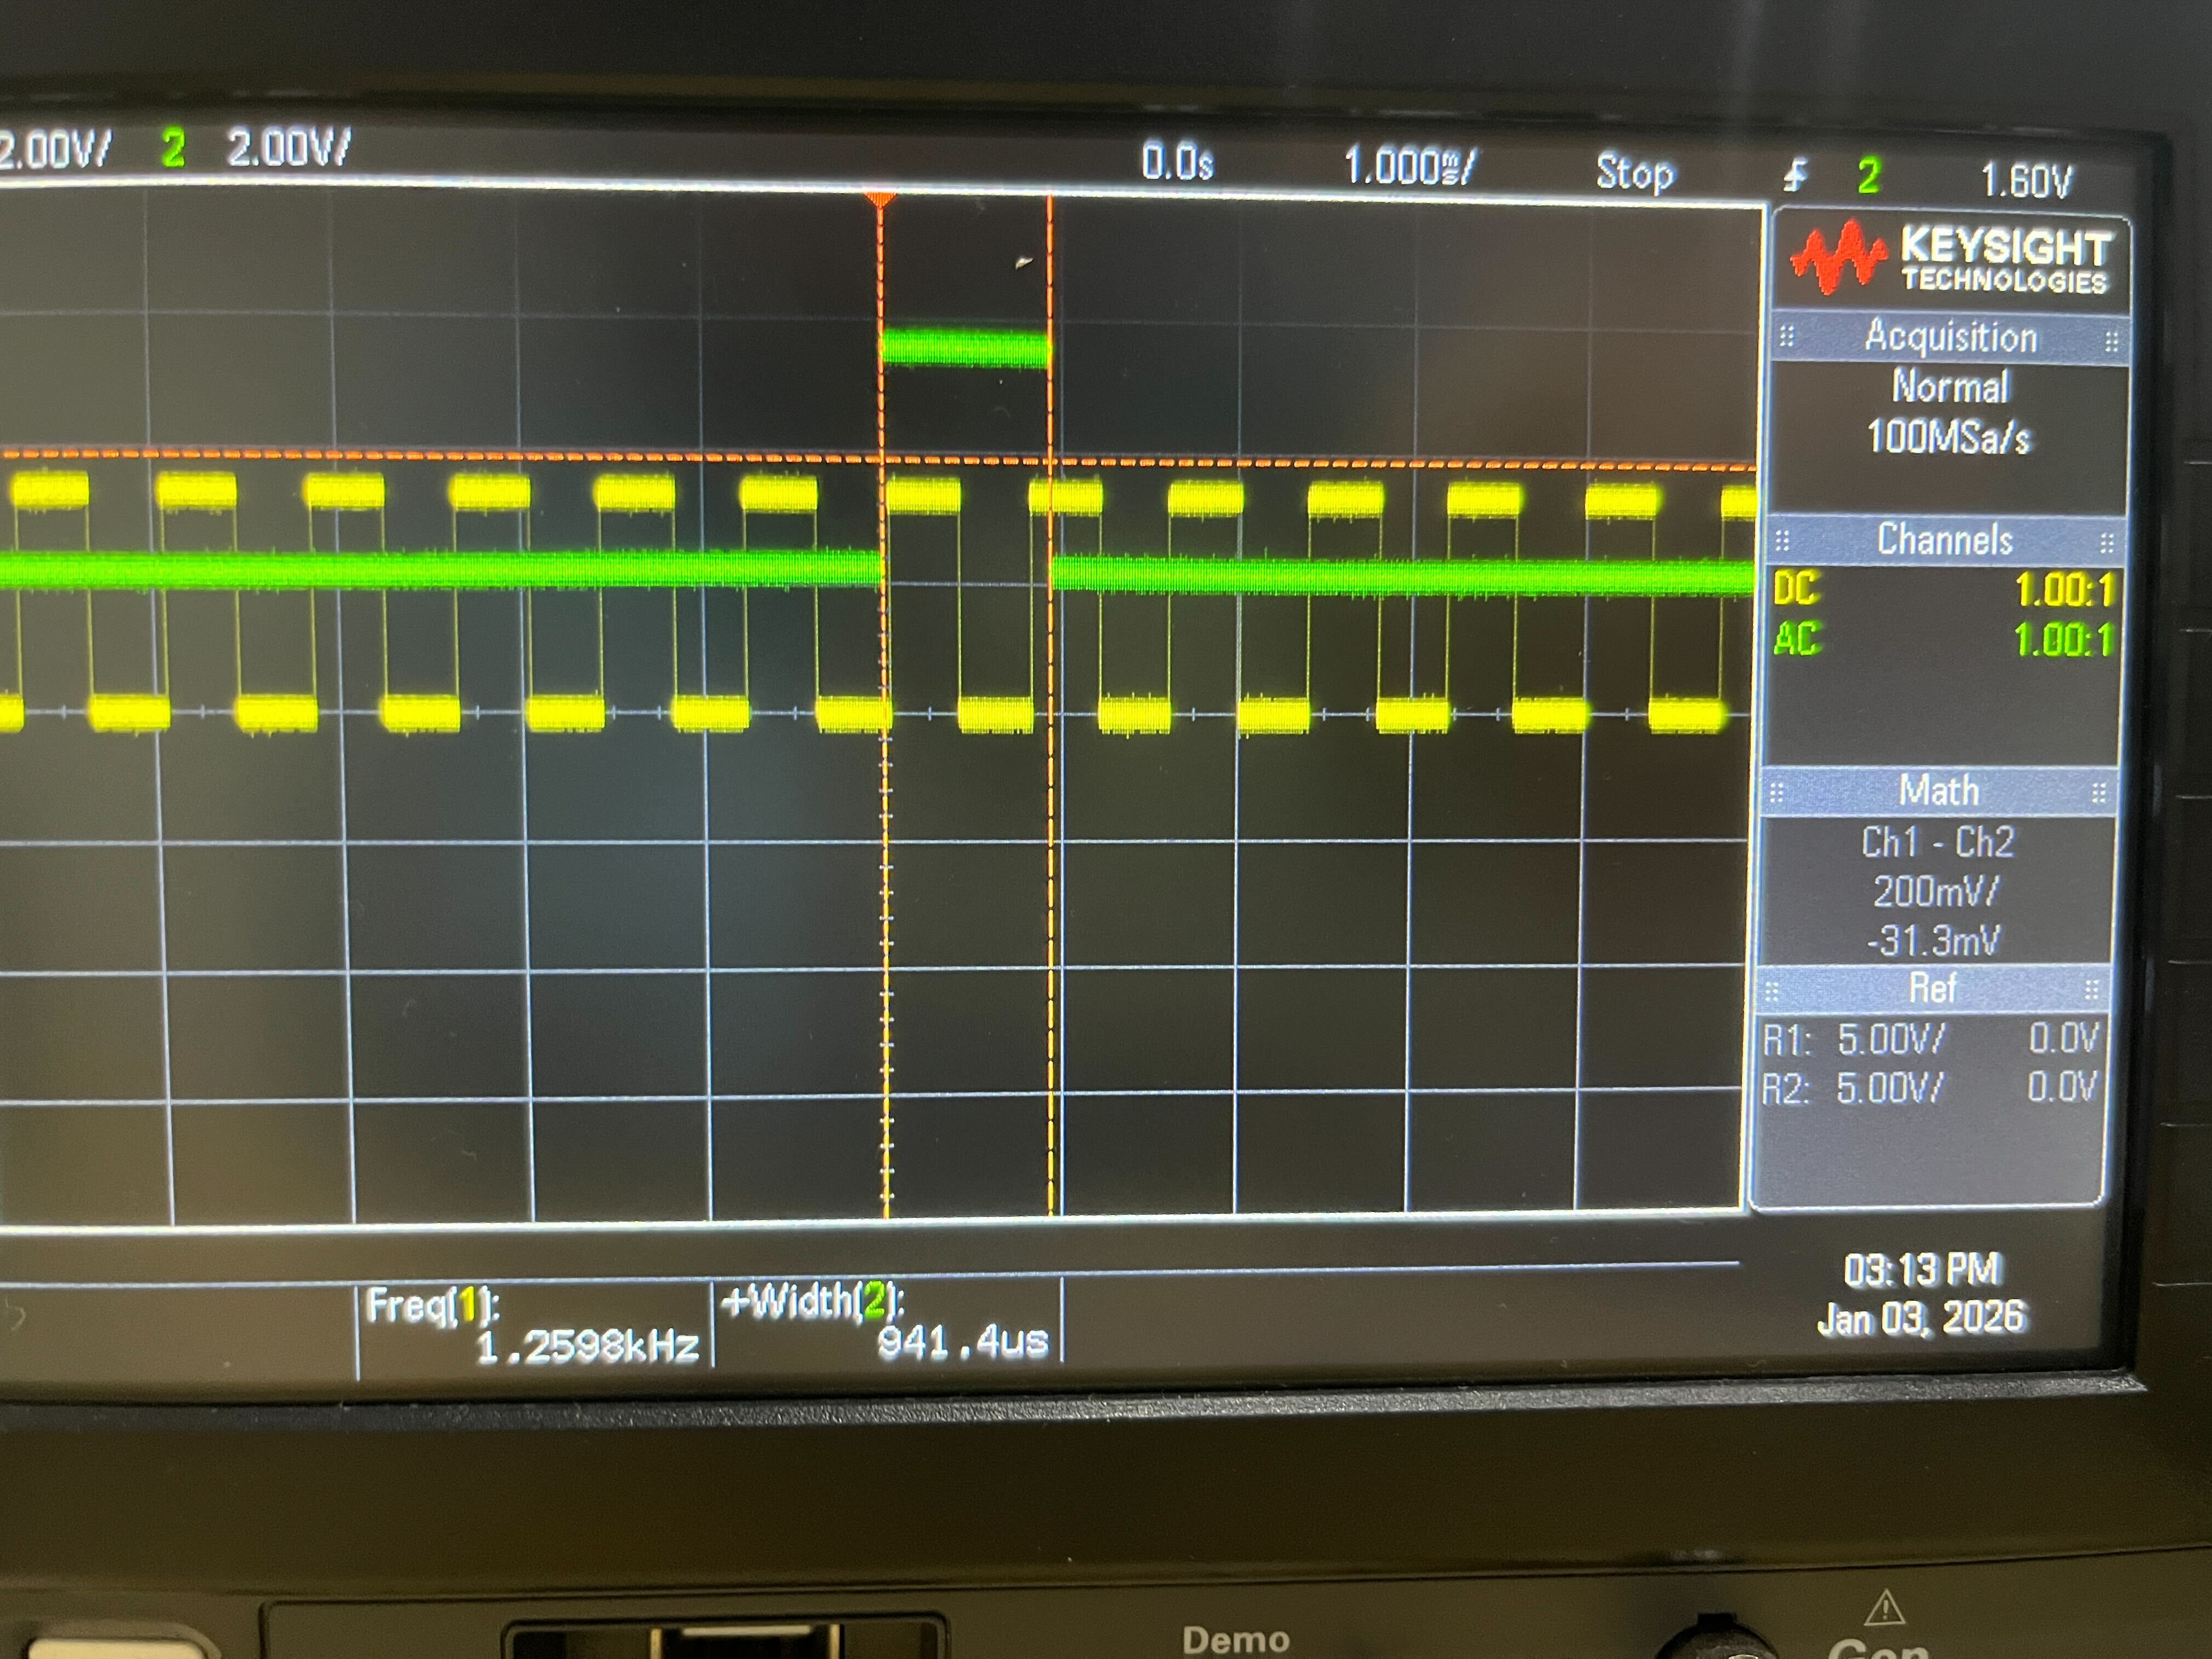
\includegraphics[width=0.45\columnwidth]{fig/echo_10.jpg}}
	\subcaptionbox{ 15cm, 1.3349kHz 
		\label{fig:buzzer_5cm}}{
		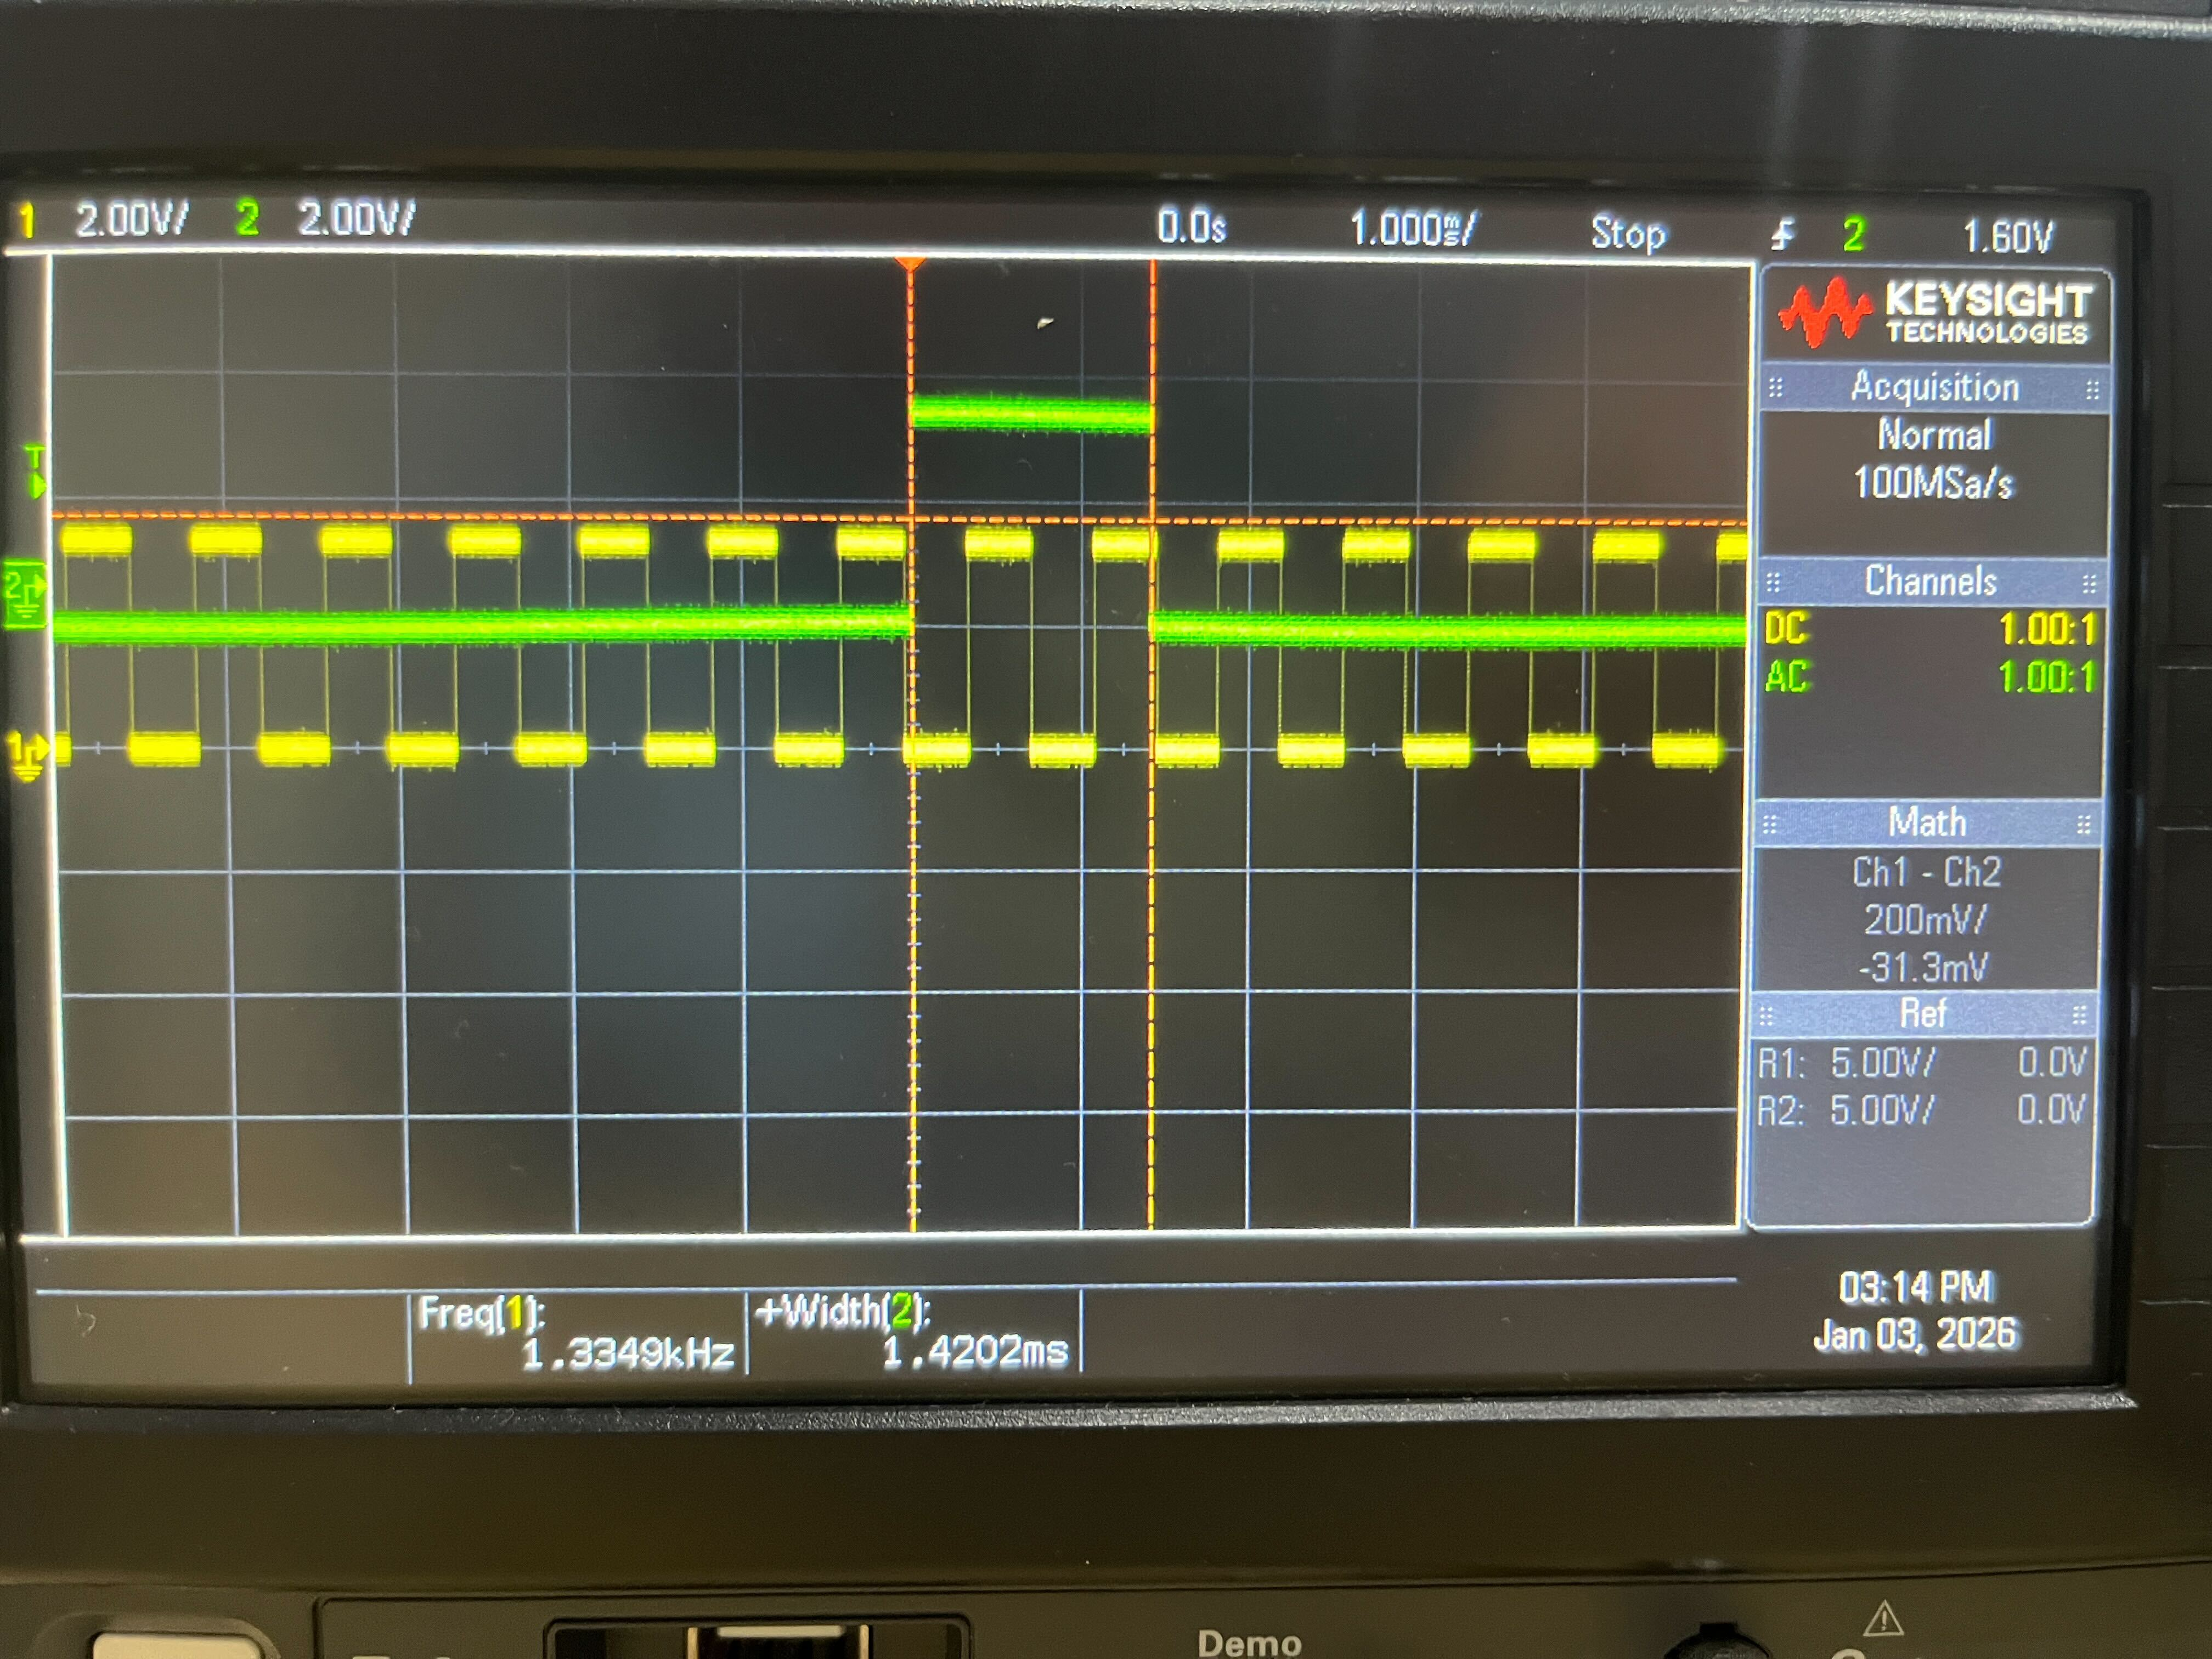
\includegraphics[width=0.45\columnwidth]{fig/echo_20.jpg}}
	\caption{Frequency change of the PWM signal (yellow wave). 
  We can observe that different distance calculated with the echo pin signal (green wave) is inducing different frequency accordingly.}
\label{fig:buzz_dist_to_freq}
\end{figure}

\begin{lstlisting}[language=C, caption={PWM Configuration Function for Buzzer Output}, label={lst:buzzer_pwm_set}]
static fsp_err_t buzzer_pwm_set(float freq_hz, float duty_percent)
{
    /* Duty-cycle clamping */
    if (freq_hz < 1.0f)        { freq_hz = 1.0f; }
    if (duty_percent < 0.0f)   { duty_percent = 0.0f; }
    if (duty_percent > 100.0f) { duty_percent = 100.0f; }

    timer_info_t info = {0};
    fsp_err_t err = R_GPT_InfoGet(&g_timer11_ctrl, &info);
    if (FSP_SUCCESS != err) { return err; }

    uint32_t clk = info.clock_frequency;
    if (clk == 0U) { return FSP_ERR_INVALID_ARGUMENT; }

    /* Minimum frequency clamp due to 16-bit period limit */
    float f_min_hw = (float) clk / (float) (GPT11_MAX_PERIOD_COUNTS + 1U);
    if (freq_hz < f_min_hw)
    {
        freq_hz = f_min_hw;
    }

    /* Compute timer period from desired frequency */
    float ticks_per_cycle_f = (float) clk / freq_hz;
    if (ticks_per_cycle_f < 2.0f)
    {
        ticks_per_cycle_f = 2.0f;
    }

    uint32_t ticks_per_cycle = (uint32_t) (ticks_per_cycle_f + 0.5f);
    if (ticks_per_cycle < 2U) { ticks_per_cycle = 2U; }

    uint32_t period_counts = ticks_per_cycle - 1U;
    if (period_counts > GPT11_MAX_PERIOD_COUNTS)
    {
        period_counts = GPT11_MAX_PERIOD_COUNTS;
    }

    /* Duty-cycle conversion */
    uint32_t duty_counts =
        (uint32_t) ((float) (period_counts + 1U) * (duty_percent / 100.0f));

    if (duty_counts == 0U)
    {
        duty_counts = 1U;
    }
    if (duty_counts >= (period_counts + 1U))
    {
        duty_counts = period_counts;
    }

    /* Apply configuration */
    (void) R_GPT_Stop(&g_timer11_ctrl);

    err = R_GPT_PeriodSet(&g_timer11_ctrl, period_counts);
    if (FSP_SUCCESS != err) { return err; }

    err = R_GPT_DutyCycleSet(&g_timer11_ctrl,
                             duty_counts,
                             GPT_IO_PIN_GTIOCB);
    if (FSP_SUCCESS != err) { return err; }

    return R_GPT_Start(&g_timer11_ctrl);
}
\end{lstlisting}


%%%%%%%%%%%%%%%%%%%%%%%%%%%%%%%%%%%%%%%%%%%%%%%%%%%%%%%%%%%%%%%%%%
\section{Main Control Flow Implementation}
%%%%%%%%%%%%%%%%%%%%%%%%%%%%%%%%%%%%%%%%%%%%%%%%%%%%%%%%%%%%%%%%%%


\begin{figure}[H]
	\centering
		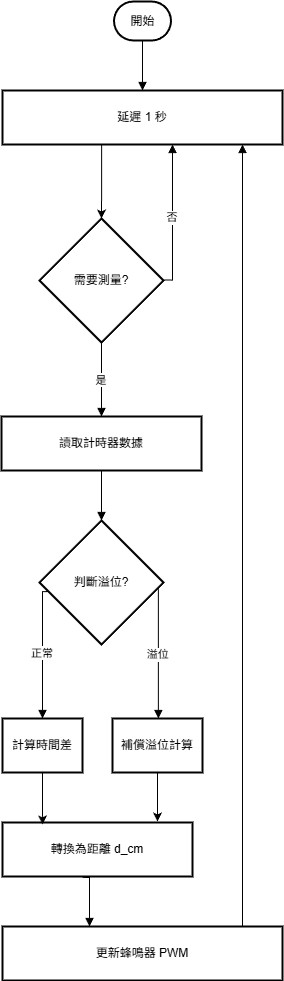
\includegraphics[width=0.25\columnwidth]{fig/hal_entry_flow.png}
	\caption{Control flow of the main function}
\label{fig:hal_entry_flow}
\end{figure}

\pagebreak



%%%%%%%%%%%%%%%%%%%%%%%%%%%%%%%%%%%%%%%%%%%%%%%%%%%%%%%%%%%%%%%%%%
\section{Distance Error Source Analysis}
%%%%%%%%%%%%%%%%%%%%%%%%%%%%%%%%%%%%%%%%%%%%%%%%%%%%%%%%%%%%%%%%%%


We perform a similar error calibration as in the previous experiment.
Firstly, since we're using the same module, we reconducted the distance measurement comparing to the theoretical transformation equations.
\begin{table}[h!]
\centering
\caption{Relative Distance Comparison (Measured vs. Theoretical)}
\begin{tabular}{|c|c|c|c|c|c|c|}
\hline
Pair (cm) & $n^*_{\mathrm{theory}}$ & $n_{\mathrm{meas}}$ &
$\Delta n^*_{\mathrm{theory}}$ & $\Delta n_{\mathrm{meas}}$ &
$\frac{\Delta n_{\mathrm{meas}}}{\Delta n^*_{\mathrm{theory}}}$ &
Relative Error (\%) \\
\hline
20$\rightarrow$40 & 184.97$\rightarrow$369.94 & 231$\rightarrow$412 & 184.97 & 181 & 0.979 & $-2.1$ \\
40$\rightarrow$60 & 369.94$\rightarrow$554.91 & 412$\rightarrow$598 & 184.97 & 186 & 1.006 & $+0.6$ \\
60$\rightarrow$80 & 554.91$\rightarrow$739.88 & 598$\rightarrow$773 & 184.97 & 175 & 0.946 & $-5.4$ \\
80$\rightarrow$100 & 739.88$\rightarrow$924.86 & 773$\rightarrow$953 & 184.97 & 180 & 0.973 & $-2.7$ \\
\hline
\end{tabular}
\end{table}

The measured peak indices $n_{\mathrm{meas}}$ were aligned relative to the start of transmission, determined by the maximum slope of the Tx waveform. We then plotted $n_{\mathrm{meas}}$ against $n^*$, as well as the corresponding sample index error $\Delta n = n_{\mathrm{meas}} - n^*$, as shown below.

\begin{figure}[!h]
	\centering
	\subcaptionbox{Measured peak index and theoretical $n^*$
		\label{fig:sample_meas_theo}}{
		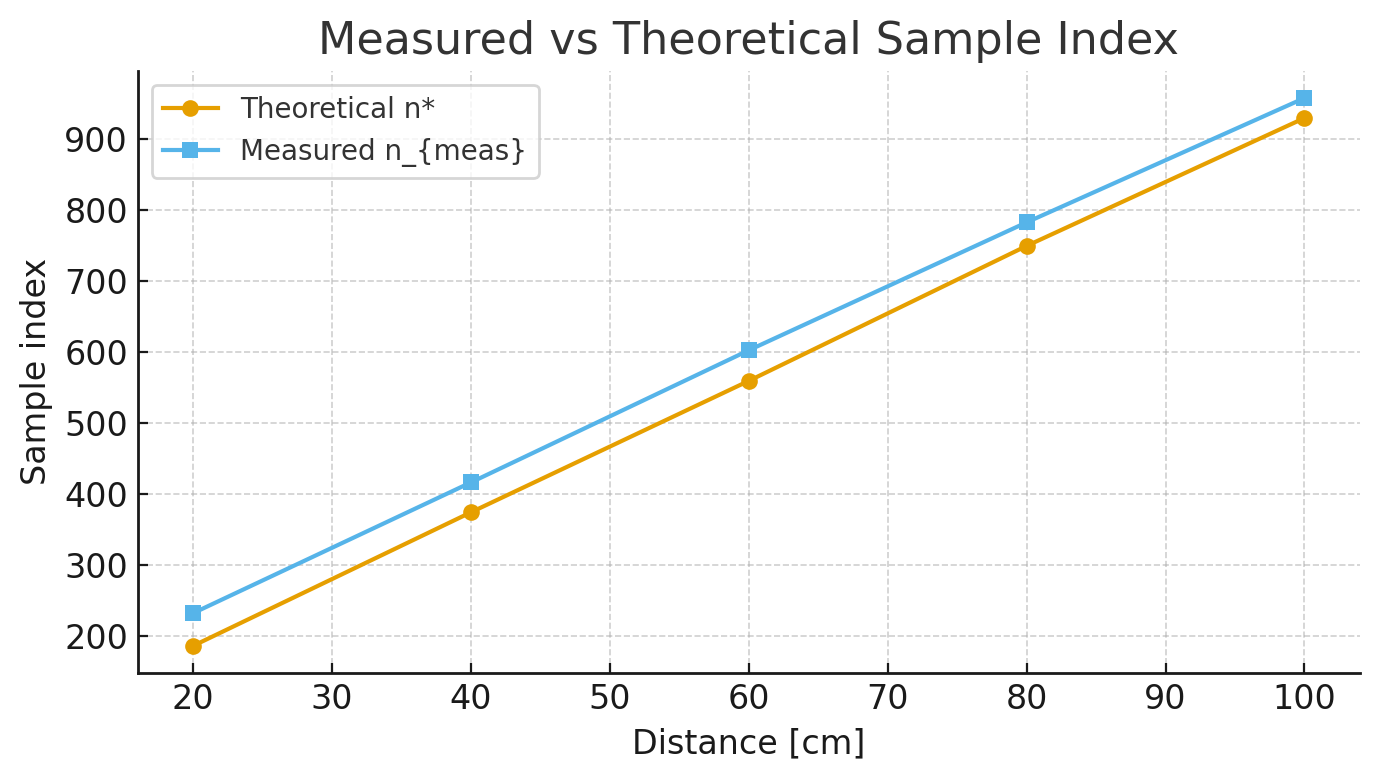
\includegraphics[width=0.45\columnwidth]{fig/distance_vs_sample_theo_meas.png}}
	\subcaptionbox{Sample index error vs. distance%
		\label{fig:error_vs_dist}}{
		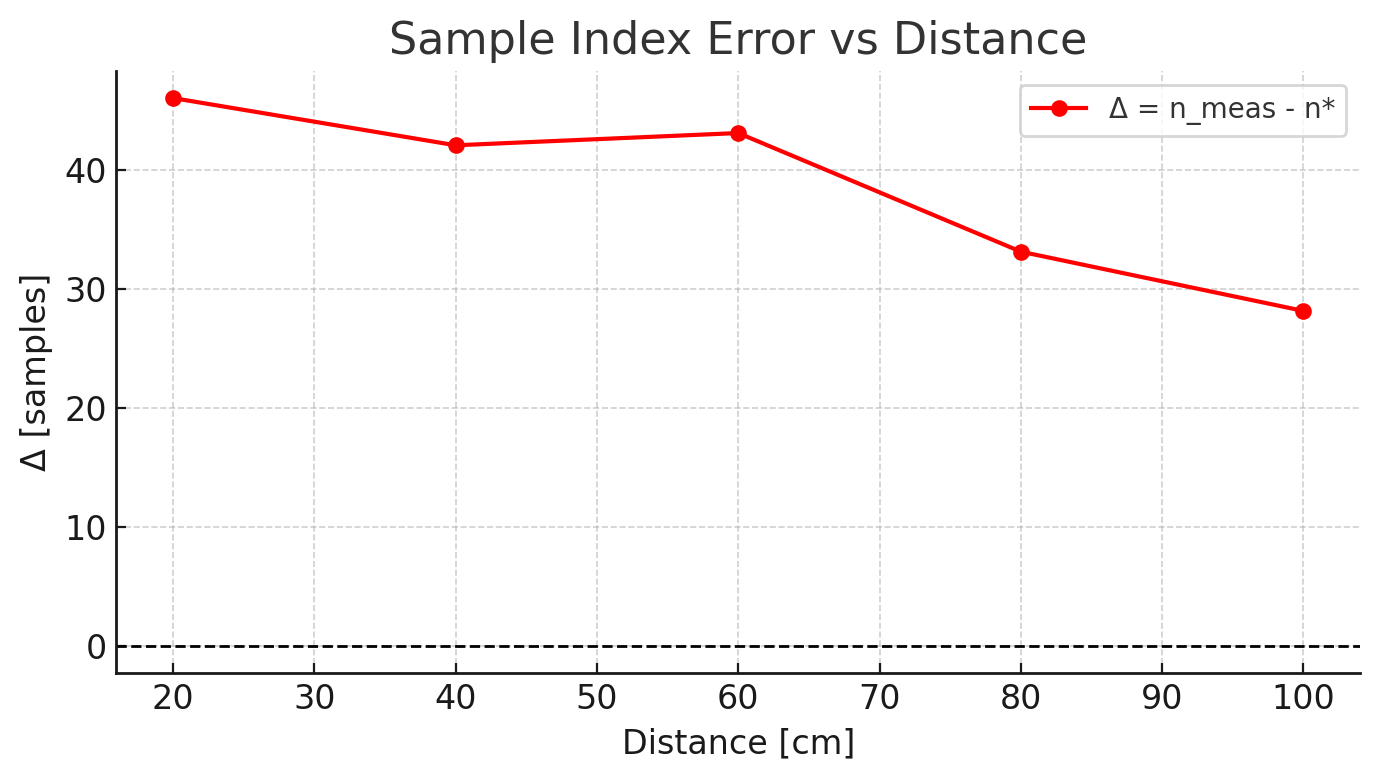
\includegraphics[width=0.45\columnwidth]{fig/distance_vs_delta.png}}
	\caption{Comparison between measured peak indices and theoretical sample indices.}
\label{fig:robust_lin}
\end{figure}

From Fig.~\ref{fig:error_vs_dist}, we observe that the error $\Delta n$ decreases approximately linearly as distance increases, 
consistent with a fixed system delay plus a small distance-dependent effect. 
Instead of the usual choice of a constant model, we found out that the error is related to the distance. 
We therefore model the error as

\[
\Delta n = a + b\,n_{\mathrm{meas}},
\]

and use linear regression to estimate $a \simeq 53.14$ and $b \simeq -0.02469$. Applying this model, we compute corrected sample indices $\hat{n} = n_{\mathrm{meas}} - \Delta n$, yielding the results summarized below.

\begin{table}[h!]
\centering
\caption{Corrected Sample Index and Residual Distance Error (Linear Model)}
\begin{tabular}{|c|c|c|c|c|}
\hline
True Distance (cm) & $n_{\mathrm{meas}}$ & $\hat{n}$ (Corrected) & $n^{*}$ (Theory) & Error After Correction (cm) \\
\hline
20  & 231 & 183.56 & 184.97 & $-0.15$ \\
40  & 412 & 369.04 & 369.94 & $-0.10$ \\
60  & 598 & 559.39 & 554.91 & $+0.48$ \\
80  & 773 & 738.65 & 739.88 & $-0.13$ \\
100 & 953 & 922.23 & 924.86 & $-0.28$ \\
\hline
\end{tabular}\label{tab:corrected_indices}
\end{table}

The corrected indices significantly reduce the bias, with all residual distance errors falling within $\pm 0.5\ \mathrm{cm}$, demonstrating that the linear error model is effective.

To translate the measured sample index back into a physical distance, we use the relation between
the sample index $n$, the sampling frequency $F_s$, and the speed of sound $v$.
Each sample corresponds to a time increment of
\[
T_s = \frac{1}{F_s},
\]
so the round-trip time corresponding to $n$ samples is
\[
t = n \, T_s = \frac{n}{F_s}.
\]

Assuming a two-way (Tx–Rx) propagation path, the one-way distance is then given by
\[
\hat{d} = \frac{v \, t}{2} = \frac{v}{2 F_s}\, n.
\]

For our experiment at $T = 25^\circ\mathrm{C}$, we use
$v = 331 + 0.6T \approx 346\ \mathrm{m/s} = 34{,}600\ \mathrm{cm/s}$ and
$F_s = 160\ \mathrm{kHz}$, which yields the conversion factor
\[
k = \frac{v}{2F_s}
= \frac{34{,}600}{2 \times 160{,}000}
\simeq 0.1081\ \frac{\mathrm{cm}}{\mathrm{sample}}.
\]

Thus, the estimated distance from a measured sample index $n_{\mathrm{meas}}$ (or its corrected version $\hat{n}$) is
\[
\hat{d} = k \, n.
\]

This linear relation allows us to directly convert the corrected sample indices from
Table~\ref{tab:corrected_indices} into absolute distance estimates and to compute residual
errors in centimeters for performance evaluation.


To fully exploit our calibration, we convert our measured width to corresponding number of samples using $F_s = 160kHz$
\begin{table}[h!]
\centering
\caption{Relative Distance Comparison (Measured vs. Theoretical)}
\begin{tabular}{|c|c|c|c|}
\hline
distance(cm) & width($\mu s$) & sample(n) & $\hat{d}$(cm)\\
\hline
5   & 327.5 &  52& 5.66\\
10  & 620.8 &  99&10.74\\
15  & 941.4 & 151&16.28\\
20  & 1205.5& 193&20.85\\
23  & 1240.2& 198&21.45\\
30  & 1848.9& 296&31.97\\
\hline
\end{tabular}
\end{table}

\section{Music Scale Discretization}

We initially try to make the scale flexible as the true Theremin, but we found out that it will make it 
so hard to play and we really don't have that much of time to practice playing such a naive instrument. 
Therefore, we decided to make the scale discrete to give us some flexibility.


\begin{lstlisting}[language=C, caption={Distance-to-Frequency Mapping Quantized to C Major Scale}, label={lst:distance_to_freq}]
static float distance_to_freq_hz(float d_cm)
{
    /* Continuous inverse mapping */
    d_cm = clampf(d_cm, D_MIN_CM, D_MAX_CM);
    float inv = 1.0f / d_cm;
    float inv_min = 1.0f / D_MAX_CM;
    float inv_max = 1.0f / D_MIN_CM;

    float t = (inv - inv_max) / (inv_min - inv_max);
    t = clampf(t, 0.0f, 1.0f);

    float f_cont = F_MIN_HZ + (F_MAX_HZ - F_MIN_HZ) * t;

    /* Quantize to C major scale between F_MIN_HZ and F_MAX_HZ */
    const float f_base = F_MIN_HZ;
    float best_f = F_MIN_HZ;
    float best_err = 1e30f;

    for (int octave = 0; octave < 8; ++octave)
    {
        int octave_offset = 12 * octave;

        for (int i = 0; i < 7; ++i)
        {
            int semitone = octave_offset + k_major_steps[i];
            float f = f_base * powf(2.0f, (float) semitone / 12.0f);

            if (f < F_MIN_HZ) { continue; }
            if (f > F_MAX_HZ) { break; }

            float err = fabsf(f - f_cont);
            if (err < best_err)
            {
                best_err = err;
                best_f = f;
            }
        }
    }

    return best_f;
}
\end{lstlisting}


\section{Digital Theremin}

\begin{figure}[H]
	\centering
		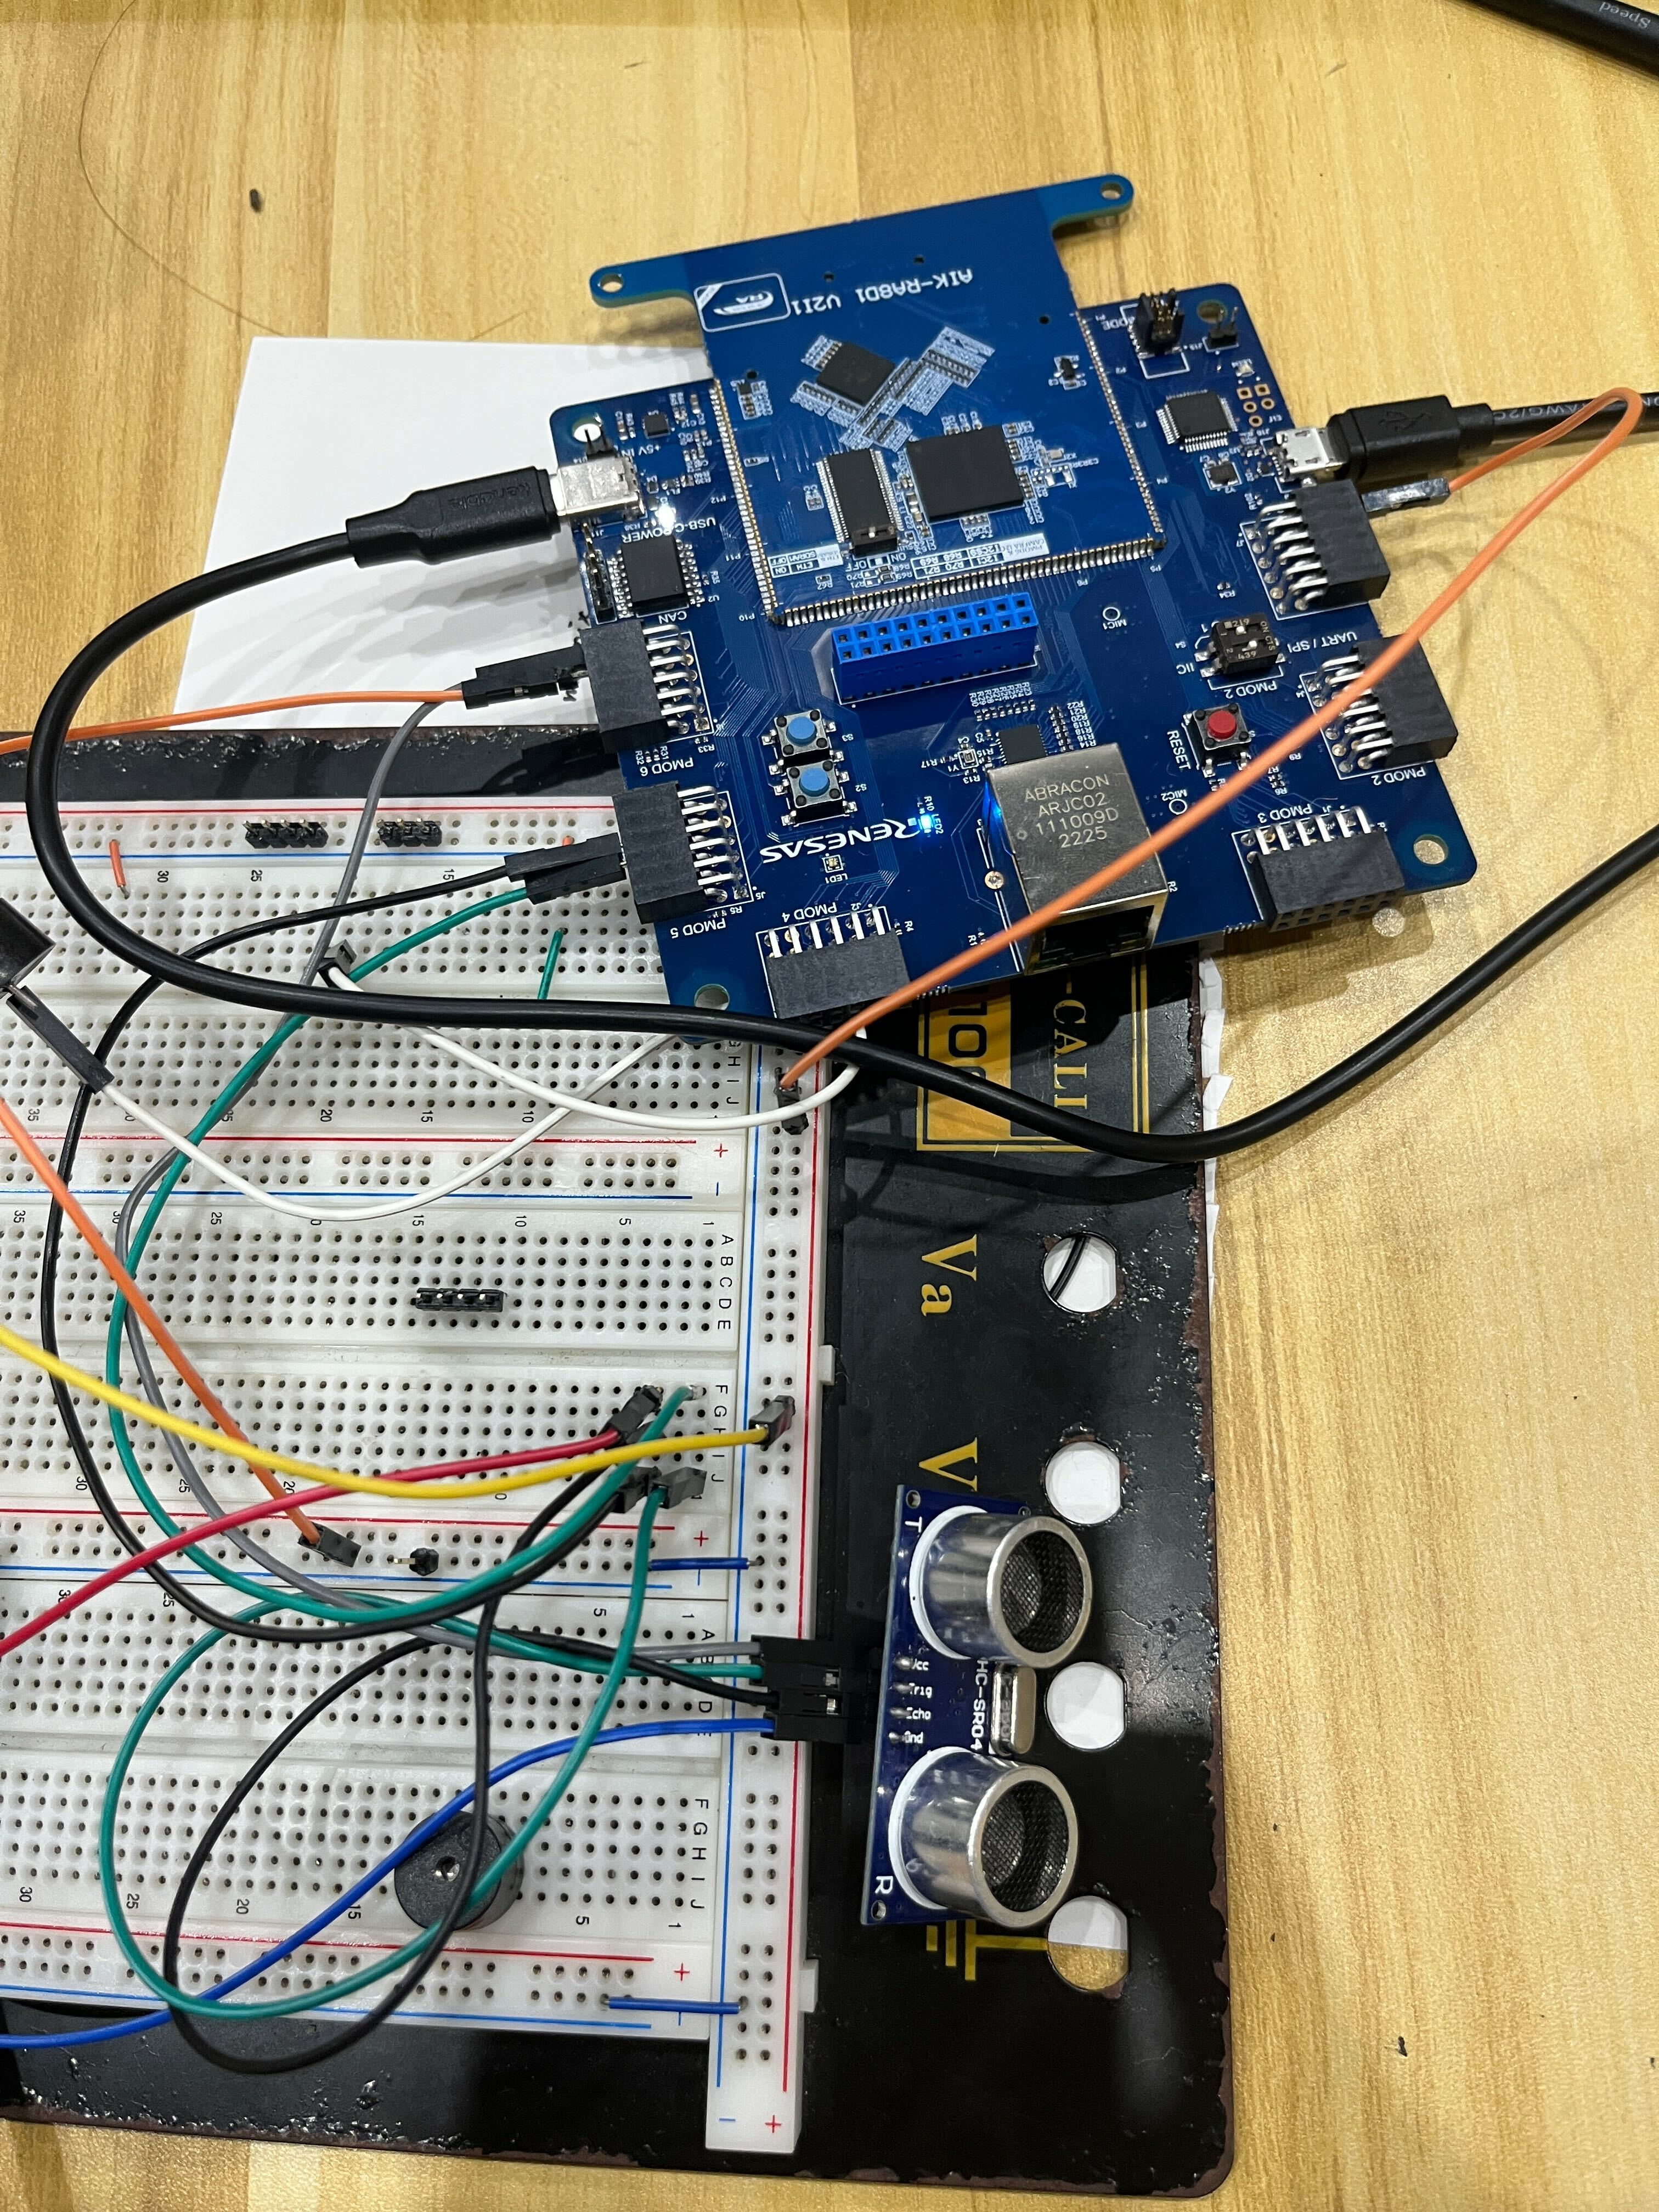
\includegraphics[width=0.75\columnwidth]{fig/renessas_MCU_theremin.jpg}
	\caption{Final Implementation. We are really proud of actually making it work.}
\label{fig:MCU}
\end{figure}

\section{Quantized Scale to MIDI and PC Logging}
\label{sec:midi_impl}

This section describes how the quantized pitch (C major scale) can be converted into MIDI note messages and saved on a host computer as a standard MIDI file (\texttt{.mid}). The implementation is split into two parts: (i) generating MIDI events on the MCU and streaming them to the host, and (ii) recording the stream and writing a MIDI file on the PC.

\subsection{MCU-Side: Frequency-to-MIDI and Serial Streaming}
\label{subsec:mcu_midi}

\subsubsection{Mapping Quantized Frequency to a MIDI Note Number}

After \texttt{distance\_to\_freq\_hz()} returns a quantized frequency $f$ (in Hz), the corresponding MIDI note number is computed using the equal-tempered formula
\[
n = \mathrm{round}\!\left(69 + 12 \log_2\!\left(\frac{f}{440}\right)\right),
\]
where MIDI note 69 corresponds to A4 = 440 Hz.

\subsubsection{MIDI Message Format}

A MIDI Note On event is a 3-byte message:
\[
\texttt{0x90},\; \texttt{note},\; \texttt{velocity}
\]
and Note Off can be sent as either \texttt{0x80} or \texttt{0x90} with velocity 0:
\[
\texttt{0x90},\; \texttt{note},\; \texttt{0x00}.
\]

In this project, we transmit raw MIDI bytes over a serial link (USB CDC or UART). The host PC interprets the incoming bytes and logs them into a MIDI file.

\subsubsection{Reference Implementation (MCU)}

\begin{lstlisting}[language=C, caption={MCU-side: Convert Frequency to MIDI Note and Stream Note Events}, label={lst:mcu_midi}]
#include <math.h>
#include <stdint.h>
#include <stdbool.h>

#ifndef M_PI
#define M_PI 3.14159265358979323846
#endif

static inline float log2f_compat(float x)
{
    return logf(x) / logf(2.0f);
}

static inline uint8_t clamp_u8(int v)
{
    if (v < 0)   return 0;
    if (v > 127) return 127;
    return (uint8_t) v;
}

static uint8_t freq_to_midi_note(float f_hz)
{
    float n = 69.0f + 12.0f * log2f_compat(f_hz / 440.0f);
    int note = (int) lroundf(n);
    return clamp_u8(note);
}

static void midi_stream_write_bytes(const uint8_t *buf, uint32_t len);

static void midi_note_on(uint8_t note, uint8_t velocity)
{
    uint8_t msg[3] = { 0x90, note, velocity };
    midi_stream_write_bytes(msg, 3);
}

static void midi_note_off(uint8_t note)
{
    uint8_t msg[3] = { 0x90, note, 0x00 };
    midi_stream_write_bytes(msg, 3);
}

static uint8_t g_last_note = 0xFF;

void buzzer_note_update_from_distance(float d_cm)
{
    float f_hz = distance_to_freq_hz(d_cm);   /* quantized to C major */
    uint8_t note = freq_to_midi_note(f_hz);

    if (note != g_last_note)
    {
        if (g_last_note != 0xFF)
        {
            midi_note_off(g_last_note);
        }

        midi_note_on(note, 90);

        g_last_note = note;
    }
}
\end{lstlisting}

The function \texttt{buzzer\_note\_update\_from\_distance()} can be called at the same point where PWM frequency is updated. Instead of generating sound purely via PWM, the MCU emits MIDI note events that can be synthesized or recorded on the host.

\subsection{PC-Side: Capture Stream and Save to a MIDI File}
\label{subsec:pc_midi}

\subsubsection{Design}

The host PC reads the raw MIDI bytes coming from the serial port and reconstructs note events. These events are timestamped and stored into a standard MIDI track, then written to \texttt{output.mid}. This allows later playback in any DAW or MIDI player.

\subsubsection{Reference Implementation (Python)}

The following script uses:
\begin{itemize}
    \item \texttt{pyserial} for reading from a serial device, and
    \item \texttt{mido} for writing a MIDI file.
\end{itemize}

\begin{lstlisting}[language=Python, caption={PC-side: Read MIDI Bytes from Serial and Save as \texttt{.mid}}, label={lst:pc_midi}]
import time
import serial
import mido

PORT = "COM5"         
OUT_MID = "output.mid"

# Simple 3-byte MIDI parser for Note On/Off on channel 1
def read_midi_messages(ser):
    buf = bytearray()
    while True:
        data = ser.read(ser.in_waiting or 1)
        if data:
            buf.extend(data)

        # Parse 3-byte messages: status, note, vel
        while len(buf) >= 3:
            status, note, vel = buf[0], buf[1], buf[2]
            if status in (0x90, 0x80):
                yield (status, note, vel)
                del buf[:3]
            else:
                # Resync: drop one byte
                del buf[0]

def main():
    ser = serial.Serial(PORT, BAUD, timeout=0.01)

    mid = mido.MidiFile(ticks_per_beat=480)
    track = mido.MidiTrack()
    mid.tracks.append(track)

    tempo = mido.bpm2tempo(120)  # 120 BPM
    track.append(mido.MetaMessage("set_tempo", tempo=tempo, time=0))

    last_t = time.time()

    print("Recording... Press Ctrl+C to stop.")
    try:
        for status, note, vel in read_midi_messages(ser):
            now = time.time()
            dt_sec = now - last_t
            last_t = now

            # ticks = dt_sec * (ticks_per_beat * beats_per_second)
            bps = 120 / 60.0
            ticks = int(dt_sec * mid.ticks_per_beat * bps)

            if status == 0x90 and vel > 0:
                msg = mido.Message("note_on", note=int(note), velocity=int(vel), time=ticks)
            else:
                msg = mido.Message("note_off", note=int(note), velocity=0, time=ticks)

            track.append(msg)

    except KeyboardInterrupt:
        pass
    finally:
        ser.close()

    mid.save(OUT_MID)
    print(f"Saved: {OUT_MID}")

if __name__ == "__main__":
    main()
\end{lstlisting}

This logger produces a valid MIDI file that preserves the temporal structure of the note events emitted by the MCU. The resulting \texttt{output.mid} can be imported into any MIDI-capable audio environment for playback or further analysis.

\begin{figure}[H]
	\centering
		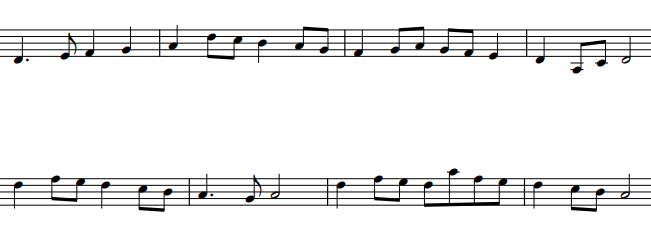
\includegraphics[width=0.75\columnwidth]{fig/MIDI.png}
	\caption{The Exported MIDI file opened in Musescore4}
\label{fig:MIDI}
\end{figure}

\section{Acknowlegdement}
We appreciate all the support from the Renessas Team, espectially the engineers Steven and Henry, 
and thanks to Hedy for the effective and responsive communication and schedule coordination.
Also, thanks for all the TAs for your kind support. 
Through all the rough time trying to make this project work, we are always grateful for Prof. Jeng always being presence and giving us emotional support.  

\end{document}




